\documentclass[]{iopart}
\usepackage{graphicx, epsfig} %include figure files
\usepackage{bm}

% The following is to avoid the error that amsmath defines equation*
% (which rightly replaces the worse iopart definition)
\expandafter\let\csname equation*\endcsname\relax
\expandafter\let\csname endequation*\endcsname\relax

\usepackage[caption=false]{subfig}
\usepackage[usenames]{xcolor}

\usepackage{marvosym}
\usepackage{yfonts}
\usepackage{upgreek}
\usepackage{pdflscape}
\definecolor{linkcolor}{rgb}{0.0, 0.3, 0.5}
\definecolor{purple}{rgb}{0.7, 0.05, 0.5}
\usepackage[unicode,colorlinks=true,citecolor=linkcolor,linkcolor=linkcolor,urlcolor=linkcolor]{hyperref}
\usepackage[all]{hypcap}
\usepackage{amsmath,amsfonts,amssymb}
%\usepackage{color}
%\usepackage[usenames,dvipsnames]{xcolor}
\usepackage{bm}
\usepackage{longtable}
\usepackage[T1]{fontenc}
\usepackage[utf8]{inputenc}
\usepackage{verbatim}
\usepackage{pifont}
\usepackage{yfonts}
\usepackage{url}
\usepackage{multirow}
\usepackage{tensor}
\usepackage{mathtools}
\usepackage[normalem]{ulem}
\normalem
\usepackage{fancyhdr}
\usepackage{xcolor}
\usepackage{soul}

\renewcommand{\vec}[1]{\boldsymbol{#1}}
\newcommand{\iu}{\mathrm{i}\mkern1mu}
\newcommand{\du}{\mathrm{d}}

\newcommand{\rc}[1]{\textcolor{blue}{[{\it\textbf{RC: #1}}]} }
\newcommand{\us}[1]{\textcolor{teal}{[{\it\textbf{US: #1}}]} }
\renewcommand{\mr}[1]{\textcolor{purple}{[{\it\textbf{MR: #1}}]} }
\renewcommand{\th}[1]{\textcolor{orange}{[{\it\textbf{TH: #1}}]} }
\newcommand{\kc}[1]{\textcolor{magenta}{[{\it\textbf{KC: #1}}]} }
\newcommand{\el}[1]{\textcolor{brown}{[{\it\textbf{EL: #1}}]} }
\newcommand{\new}[1]{\textcolor{red}{#1}}
\newcommand*{\defeq}{\mathrel{\vcenter{\baselineskip0.5ex \lineskiplimit0pt
                     \hbox{\scriptsize.}\hbox{\scriptsize.}}}%
                     =}
\newcommand*{\invdefeq}{=\mathrel{\vcenter{\baselineskip0.5ex \lineskiplimit0pt
                     \hbox{\scriptsize.}\hbox{\scriptsize.}}}%
                     }

\begin{document}
\newcounter{count}

\pagestyle{fancy}\lhead{Malaise and remedy of binary boson-star initial data}
\chead{}
\rhead{\thepage}
\lfoot{}
\cfoot{}
\rfoot{}

\begin{center}
\title{\large Malaise and remedy of binary boson-star initial data}
\end{center}

\author{
Thomas Helfer$^{1}$,
Ulrich Sperhake$^{2,3}$,
Robin Croft$^{2}$,
Miren Radia$^{2}$,
Bo-Xuan Ge$^4$,
Eugene A. Lim$^4$
}

\address{$^{1}$~Department of Physics and Astronomy, Johns Hopkins University, 3400 N. Charles Street, Baltimore, Maryland 21218, USA}

\address{$^{2}$~Department of Applied Mathematics and Theoretical Physics,
Centre for Mathematical Sciences, University of Cambridge,
Wilberforce Road, Cambridge CB3 0WA, United Kingdom}

\address{$^{3}$~Theoretical Astrophysics 350-17,
California Institute of Technology,
1200 E California Boulevard, Pasadena, CA 91125, USA}

%\address{$^{4}$~Astrophysics, University of Oxford, DWB, Keble Road, Oxford OX1 3RH, UK}

\address{$^{4}$~Theoretical Particle Physics and Cosmology Group, Physics Department,Kings College London, Strand, London WC2R 2LS, United Kingdom}



\ead{U.Sperhake@damtp.cam.ac.uk}


\begin{abstract}
Through numerical simulations of boson-star head-on collisions,
we explore
the quality of binary initial data obtained from the superposition
of single-star spacetimes. 
Our results demonstrate that evolutions starting from a
plain superposition of individual boosted boson-star spacetimes
are vulnerable to significant unphysical artefacts. These
difficulties can be overcome with a simple modification of the
initial data suggested in \cite{Helfer:2018vtq} for collisions of oscillatons.
%\us{Do we need the remainder of the abstract?}
While we specifically consider massive complex scalar field boson star models up to a 6th-order-polynomial potential, we argue that this vulnerability is universal and present in other kinds of
exotic compact systems and hence needs to be addressed.
%\us{The text is nice, but do we really argue that this is
%a universal problem? I don't think we do...}
%We present numerical simulations of head-on collisions of
%equal-mass, non-spinning boson stars.
%Specifically, we consider two types of boson-star models
%in this analysis, mini boson stars composed of a massive, non-interacting
%complex scalar field, and solitonic boson stars where the scalar field
%obeys a potential also including a fourth and a sixth-order term.
%We cover a wide range of initial separations to identify the suitability
%of different constructions of the binary initial data.
%Our results
%demonstrates that plain superposition of individual boosted boson star
%spacetimes is vulnerable to unphysical artifacts and how these
%difficulties may be overcome with a simple modification of the
%initial data suggested in \cite{Helfer:2018vtq} for collisions of oscillatons.
%We extract as our main diagnostics the gravitational-waves
%radiated in the collisions and the properties of apparent horizons
%if formed.
%\th{We focus very much on Boson Stars, though these ideas might likely show improvements for other compact object? }
%\el{I'll turn the abstract around, and start by saying the main point of linear superposition is bad as soon as we could. At present, the result is only stated more than half way through the abstract and some people doesn't have the patience. maybe something like "We showed in this paper that the oft-used linear superposition ansatz for boosted BS star binaries is vulnerable to unphysical spurious artifacts, which lead significant change in the physical composition of the system. We propose a remedy etc. This is a matter of style of course!}
\end{abstract}

\maketitle

%=============================================================================
\section{Introduction}
\label{sec:intro}

% \rc{Robin adds comments using {\tt \textbackslash rc\{text\}.}}

% \noindent
% \th{Thomas adds comments using {\tt \textbackslash th\{text\}.}}

% \noindent
% \mr{Miren adds comments using {\tt \textbackslash mr\{text\}.}}

% \noindent
% \kc{Katy adds comments using {\tt \textbackslash kc\{text\}.}}

% \noindent
% \el{Eugene adds comments using {\tt \textbackslash el\{text\}.}}

% \noindent
% \us{Uli adds comments using {\tt \textbackslash us\{text\}.}}

The rise of gravitational-wave (GW) physics as an observational field,
marked by the detection of GW150914 \cite{Abbott:2016blz} and followed by about 50 further
compact binary events \cite{LIGOScientific:2018mvr,LIGOScientific:2020ibl}
over the past years, has opened
up unprecedented opportunities to explore gravitational phenomena.
From tests of general relativity
\cite{Berti:2015itd,TheLIGOScientific:2016src,Abbott:2018lct,LIGOScientific:2019fpa,LIGOScientific:2020tif,Moore:2021eok}
to the exploration
of BH populations \cite{Trifiro:2015zda,Belczynski:2017gds,LIGOScientific:2020kqk,Baibhav:2020xdf,Gerosa:2021mno}
or charting the universe with independent
new methods \cite{LIGOScientific:2017adf,LIGOScientific:2019zcs}, GW astronomy offers potential for
revolutionary insight into long-standing open questions;
for a review see \cite{Barack:2018yly}.
Some answers,
such as the association of a soft gamma-ray burst with the neutron star merger GW170817
\cite{TheLIGOScientific:2017qsa,Monitor:2017mdv} have already raised our understanding to new levels.
GW physics furthermore establishes new concrete links to other
fields of research, most notably to particle and high-energy
physics and the exploration of the dark sector of the universe
\cite{Cardoso:2014uka,Barack:2018yly}.
Two important ingredients of this remarkable connection are the
characteristic interaction of fundamental fields with compact
objects through superradiance \cite{Brito:2015oca} and their capacity
to form compact objects through an elaborate balance between
the intrinsically dispersive character of the fields and their
self-gravitation. The latter feature has given rise to the
hypothesis of a distinct class of compact objects as early as the
1950s \cite{Wheeler:1955zz}. In contrast to their well known fermionic counterparts --
stars, white dwarfs or neutron stars -- these compact objects are composed
of bosonic particles or fields and, hence, commonly referred to as
{\em Boson Stars} (BS). GW observations provide the first systematic
approach to search for populations of these objects or to constrain their
abundance. As with all other GW explorations, the success of
this exploration is heavily reliant on the availability of accurate
theoretical predictions for the anticipated GW signals.
%to be expected from these
%compact objects and the binary systems they may form.
This type of
calculation, using numerical relativity techniques
% \mr{Is this book you reviewed now the canonical numerical relativity reference?}
\cite{Baumgarte:2021skc}, is the topic of this work.

The idea of bosonic stars dates back to Wheeler's 1955 study of
gravitational-electromagnetic entities or {\it geons}
\cite{Wheeler:1955zz}.
%Even though these
%configurations do not admit genuinely stationary configurations,
%their scalar analogs, often referred to as oscillatons, admit
%compact configurations with astrophysically long life times
%\cite{Seidel:1991zh,Seidel:1993zk}. By generalizing from real to complex-valued fields,
By generalising from real to complex-valued fundamental fields,
it is even possible to obtain genuinely stationary
solutions to the Einstein-matter equations. First
established for spin 0 or scalar fields
\cite{Feinblum:1968nwc,Kaup:1968zz,Ruffini:1969qy}, this idea has more
recently been extended to spin 1 or vector (aka {\it Proca}
\footnote{Even though the term ``boson star''
generally applies to compact objects formed of any bosonic
fields, it is often used to specifically denote stars made
up of a {\it scalar} field. Stars
composed of vector fields, in contrast, are most commonly
referred to as {\it Proca} stars. Unless specified otherwise,
we shall accordingly assume the term boson star to imply
scalar-field matter.})
fields \cite{Brito:2015pxa}
as well as wider classes of scalar BSs
\cite{Alcubierre:2018ahf,Choptuik:2019zji}.
In the wake of the dramatic progress of numerical
relativity in the simulations of black holes (BHs)
\cite{Pretorius:2005gq,Campanelli:2005dd,Baker:2005vv}
(see \cite{Sperhake:2014wpa} for a review),
the modelling of BSs and binary systems involving BSs has rapidly
gathered pace.

The first BS models computed in the 1960s consisted of a
massive but non-interacting complex scalar field $\varphi$.
This class of stationary BSs,
commonly referred to as {\it mini boson stars}, consists of a 
one parameter family of ground-state
solutions characterised by the central
scalar-field amplitude that reveals a stability structure
analogous to that of Tolman-Oppenheimer-Volkoff
\cite{Tolman:1939jz,Oppenheimer:1939ne} stars:
a stable and an unstable branch of ground-state solutions are
separated by the configuration with maximal mass
\cite{Breit:1983nr,Gleiser:1988ih,Seidel:1990jh}. For each ground-state model,
there furthermore exists a countable hierarchy of
excited states with $n>0$ nodes in the scalar profile
\cite{Lee:1991ax,Jetzer:1991jr,Liddle:1992fmk}. Numerical
evolutions of these excited BSs demonstrate their unstable
character, but also reveal significant variation in the
instability time scales \cite{Balakrishna:1997ej}.

Whereas mini BS models are limited in terms of their maximum
compactness, self-interacting scalar fields
%the addition of self-interaction terms
%of the form $\lambda |\varphi|^4$ or of higher order to the
%scalar potential
can result in significantly more compact stars, even
%above that of 
denser than neutron stars
\cite{Colpi:1986ye,Lee:1986ts,Schunck:1999zu,Hartmann:2012da}. This raises the intriguing
question whether compact BS binaries may reveal themselves
through characteristic GW emission analogous to that from
BHs or NSs \cite{Bustillo:2020syj}. Recent studies
conclude that this may well be within the grasp of
next-generation GW detectors and, in the case of favourable
events, even with advanced LIGO
\cite{Sennett:2017etc,DiGiovanni:2020ror,Toubiana:2020lzd}.

One of the characteristic properties of BSs is
the quantised nature of their spin. The linearised
Einstein equations in the slow-rotation limit lead
to a two-dimensional Poisson equation that does not
admit everywhere regular solutions except for trivial
constants; in consequence BSs cannot rotate perturbatively
\cite{Kobayashi:1994qi}. By relaxing the slow-rotation
approximation, Schunck and Mielke \cite{Schunck:1996he}
computed the first (differentially) rotating BSs
and found that these solutions have an integer
ratio of angular momentum to particle number. The
structure of spinning BS models has been studied extensively
over the years \cite{Ryan:1996nk,Yoshida:1997jq,Yoshida:1997qf,Yoshida:1997nd,Schunck:1999pm,Kleihaus:2005me,Kleihaus:2007vk,Kleihaus:2011sx,Collodel:2017biu}. The quantised nature
of the angular momentum also applies to Proca and
{\it Dirac} (spin $\tfrac{1}{2}$) stars
\cite{Herdeiro:2019mbz}, but numerical studies of the formation
of rotating stars have revealed a striking difference
between the scalar and vector case: while collapsing
scalar fields shed all their angular momentum through an
axisymmetric instability, the collapse of vector fields
results in spinning Proca stars with no indication of an
instability \cite{Sanchis-Gual:2019ljs,DiGiovanni:2020ror}.
This observation is supported by analytic calculations
\cite{Dmitriev:2021utv}, but the instability
may be quenched by self-interaction
terms in the potential function or in the Newtonian limit
\cite{Siemonsen:2020hcg}.
For further reviews of the structure and dynamics of single BSs,
we note the reviews
\cite{Mielke:1997re,Mielke:2000mh,Mundim:2010hi,Liebling:2012fv}.

The first simulations of BS binaries have considered the
head-on collision of configurations with phase differences
between the constituent stars or opposite frequencies
\cite{Palenzuela:2006wp}; see also
\cite{Choptuik:2009ww,Bezares:2017mzk}.
The phase or frequency differences manifest themselves most
pronouncedly in the dynamics and GW emission at late times
around merger. These collisions result in either
a BH, a non-rotating BS or a near-annihilation of the scalar
field in the case of opposite frequencies. BS binaries
with orbital angular momentum generate a GW signal
qualitatively similar to that of BH binaries during the
inspiral phase, but exhibit a much more complex structure around
merger \cite{Palenzuela:2007dm,Palenzuela:2017kcg}.
In agreement with the above mentioned BS formation 
studies, the BS inspirals also seem to avoid the formation
of spinning BSs, although they may settle down into
single nonrotating BSs.

%BS binaries are also the focus of this work.
In spite of the
rapid progress of this field, the computation of GW templates
for BSs still lags considerably behind that of BH binaries,
both in terms of precision and coverage of the parameter space.
Clearly, the presence of the matter fields adds complexity to
this challenge, but also alleviates some of the difficulties
through
the non-singular character of the BS spacetimes. The first main goal
of our study is to highlight the substantial risk of obtaining
spurious physical results due to the use of overly simplistic
initial data constructed by plain superposition of single-BS
spacetimes. Our second main goal is to demonstrate
how an astonishingly
simple modification of the superposition procedure,
first identified by Helfer
{\it et al.}~\cite{Helfer:2018vtq} for oscillatons,
overcomes most of the problems encountered with plain
superposition. We summarise our main findings as follows.
%
\begin{list}{\rm{\bf (\arabic{count})}}{\usecounter{count}
             \labelwidth0.5cm \leftmargin1.0cm \labelsep0.2cm \rightmargin0.0cm
             \parsep0.5ex plus0.2ex minus0.1ex \itemsep0ex plus0.2ex}
  \item An adjustment of the superposition procedure, given 
  by Eq.~(\ref{eq:superposplus}), results in a significant
  reduction of the constraint violations inherent to the initial data;
  see Fig.~\ref{fig:ham}.
  %
  \item In the head-on collision of mini BS binaries with rather low compactness,
  we observe a significant drop of the radiated GW energy with increasing
  distance $d$ if we use plain superposition. This physically unexpected dependence
  on the initial separation levels off only for rather large 
  $d\gtrsim 150\,M$,
  where $M$ denotes the Arnowitt-Deser-Misner (ADM) mass
  \cite{Arnowitt:1962hi}. In contrast, the total radiated energy computed from
  the evolution of our adjusted initial data displays the expected
  behaviour over the entire studied range $75.5\,M\le d\le 176\,M$:
  a very mild increase in the radiated energy with $d$. In the limit of large
  $d \gtrsim 150\,M$, both types of simulations agree within numerical uncertainties;
  see upper panel in Fig.~\ref{fig:erad}.
  %
  \item In collisions of highly compact BSs with solitonic potentials,
  the radiated energy is largely independent of the initial separations
  for both initial data types, but for plain superposition we consistently
  obtain $\sim 10\,\%$ more radiation than for the adjusted initial data;
  see bottom panel in Fig.~\ref{fig:erad}. Furthermore,
  we find plain superposition to result in a slightly faster infall.
  The most dramatic difference, however, is the collapse into individual BHs
  of both BSs well before merger if we use plain superposition. No such collapse
  occurs if we use adjusted initial data. Rather,
  these lead to the expected near-constancy of the central scalar-field amplitude
  of the BSs throughout most of the infall; see Fig.~\ref{fig:soli_ampctr}.
  %
  \item We have verified through evolutions of single boosted BSs that the
  premature collapse into a BH is closely related to the spurious metric
  perturbation (\ref{eq:metricpert}) that arises in the plain superposition
  procedure. Artificially adding the same perturbation to a single BS
  spacetime induces an unphysical collapse of the BS that is in
  qualitative and quantitative agreement with that observed in
  the binary evolution starting with plain superposition;
  see Fig.~\ref{fig:soli_ampctr}.
\end{list}
%

The detailed derivation of these results begins
in Sec.~\ref{sec:formalism} with a review of
the formalism and the computational framework of our
%single BS and binary 
BS simulations. We discuss in more detail
in Sec.~\ref{sec:superposition} the construction of initial
data through plain superposition and our modification of this
method. In Sec.~\ref{sec:results}, we compare the dynamics
of head-on collisions of mini BSs and highly compact solitonic BS
binaries starting from both types of initial data. We note
the substantial differences in the results thus obtained
and argue why we regard the results obtained with our
modification to be correct within numerical uncertainties.
We summarise our findings
and discuss future extensions of this work in
Sec.~\ref{sec:conclusions}.

Throughout this work, we use units where the speed of light and
Planck's constant are set to unity, $c=\hbar=1$. We denote
spacetime indices by Greek letters running from 0 to 3 and
spatial indices by Latin indices running from 1 to 3.

%\us{Need paragraph reviewing the most important work here.
%For now I do bullet points.}
%%
%\begin{itemize}
%  \item Seidel, Suen \cite{Seidel:1990jh,Seidel:1991zh} and Balakrishna et al.
%   \cite{Balakrishna:1997ej}: Single excited BH evolutions;
%   Kaup limit separates stable and unstable branches.
%   \item Balakrishna et al. \cite{Balakrishna:2006ru}: Similar study but
%   with 3+1 evolutions.
%   \item Balakrishna et al. \cite{Balakrishna:2007mr}: Similar study for oscillatons;
%   harder to find gauge, but similar physical behaviour.
%   \item Sanchis-Gual et al. \cite{Sanchis-Gual:2019ljs}: 3D BS and Proca star
%   evolutions. nonaxisymmetric instability for BSs, but not Proca stars.
%   \item Palenzuela et al. \cite{Palenzuela:2006wp}: Head-on BS collisions
%   with different phases or opposite frequencies have very different late-time
%   behaviour and GW output.
%   \item Palenzuela et al. \cite{Palenzuela:2007dm,Palenzuela:2017kcg}: Orbiting
%   BS binaries; inspiral GW signal fiarly simple, but
%   complex behaviour around merger, as it settles down into
%   a nonrotating BS.
%   \item Liebling, Palenzuela \cite{Liebling:2012fv}: LRR.
%   \item Mundim's PhD \cite{Mundim:2010hi}: Numerical BS evolutions; inspiral
%   for up to two orbits (major progress at the time).
%   \item Colpi, Wasserman \cite{Colpi:1986ye}: They found that self-interaction
%   can give much more compact BSs.
%   \item Schunck, Mielke \cite{Schunck:1996he}: First differentially rotating BSs;
%   integer ratio angular momentum to particle number.
%   \item Sennett et al. \cite{Sennett:2017etc}: Estimate how well LIGO and 3G
%   detectors may measure tidal deformation of BSs. Distinction from BH or NS
%   binaries possible for high masses or mass ratios with aLIGO. 3G should
%   distinguish the lot.
%   \item Valdez-Alvaro et al. \cite{ValdezAlvarado:2012xc}:
%   Single stars with fermionic and bosonic fields. Similar structure
%   of stable/unstable branches.
%   \item Yoshida, Eriguchi \cite{Yoshida:1994xi}: QNMs of BSs. Short damping time
%   scale of oscillations compared with fluid stars.
%   \item Kobayashi et al. \cite{Kobayashi:1994qi}: BSs cannot rotate
%   perturbatively. They argue that vortex lines will form for rapid roations (?).
%   \item Gleiser \cite{Gleiser:1988rq}: a $\lambda \varphi^4$ term in the
%   potential can give rise to much denser yet stable stars than mini BSs.
%   \item Gleiser, Watkins \cite{Gleiser:1988ih}: Analytic and numerical
%   proof of the stability threshold at the Kaup limit.
%   \item Bezares et al. \cite{Bezares:2017mzk}: Head-on
%   of BSs and BS-anti-BS binaries. End product is a BS
%   or near annihilation of the BSaBS pair. Orbiting BSs
%   instead form a bar that relaxes into a nonspinning BS.
%   \item Choptuik et al. \cite{Choptuik:2019zji}:
%   multi-oscillating BSs.
%   \item Collodel et al. \cite{Collodel:2017biu}:
%   Analyze excited rotating single-BS models.
%   \item Alcubierre et al. \cite{Alcubierre:2018ahf}:
%   $\ell$ boson stars. \cite{Alcubierre:2019qnh,Alcubierre:2021mvs}: Spherically
%   symmetric evolution of $\ell$ BSs; same stability branches
%   as for normal BSs. \cite{Ontanon:2021hbg}: 3+1 code for
%   computing stationary rotating BSs.
%   \item Sanchis-Gual et al. \cite{Sanchis-Gual:2020mzb}:
%   BSs head-ons can form grav.atoms.
% \end{itemize}
% %



%=============================================================================
\section{Formalism}
\label{sec:formalism}

%=============================================================================
\subsection{Action and covariant field equations}
%
The action for a complex scalar field $\varphi$ minimally coupled to gravity is given by
%
\begin{equation}
S = \int\sqrt{-g}\left\{
  \frac{1}{16\pi G}R - \frac{1}{2}\left[ 
  g^{\mu \nu}\nabla_{\mu}\bar{\varphi}\nabla_{\nu}\varphi
  + V(\varphi)\right] \right\} \du^4 x\,,
  \label{eq:action}
\end{equation}
%
where $g_{\alpha\beta}$ denotes the spacetime metric and $R$ the
Ricci scalar associated with this metric. The characteristics
of the resulting BS models depend on the scalar potential
$V(\varphi)$; in this work, we consider {\it mini boson stars}
and {\it solitonic boson stars}, obtained respectively
for the potential functions
%
\begin{equation}
  V_{\rm min} = \mu^2 |\varphi|^2\,,~~~~~~~~~~
  V_{\rm sol} = \mu^2 |\varphi|^2\left(1-2\frac{|\varphi|^2}{\sigma_0^2}
  \right)^2\,.
  \label{eq:pot}
\end{equation}
%
Here, $\mu$ denotes the mass of the scalar field and $\sigma_0$
describes the self-interaction in the solitonic potential
which can result in highly compact stars
\cite{Lee:1986ts}. Note that $V_{\rm sol}\rightarrow 
V_{\rm min}$ in the limit $\sigma_0\rightarrow \infty$.

Variation of the action (\ref{eq:action}) with respect to the
metric and the scalar field yield the Einstein and matter
evolution equations
%
\begin{eqnarray}
  &&G_{\alpha\beta} = 8\pi G T_{\alpha\beta}
  = 8\pi G\left[
  \partial_{(\alpha}\bar{\varphi}\partial_{\beta)}\varphi
  -\frac{1}{2}g_{\alpha\beta}
  \big(
  g^{\mu\nu}\partial_{\mu}
  \bar{\varphi}\partial_{\nu}\varphi+ V(\varphi)
  \big)
  \right]\,, \label{eq:Einstein} \\
  &&\nabla^{\mu}\nabla_{\mu}\varphi = \varphi V'
  \defeq \varphi \frac{\du}{\du |\varphi|^2}
  V\,.
  \label{eq:Boxvarphi}
\end{eqnarray}
%
Readers who are mainly interested in the results of our work
and/or are familiar with the equations governing BS spacetimes
may proceed directly to Sec.~\ref{sec:superposition}.

%\th{I think the rest of this section should be moved to appendix?}
%\us{The problem with that is that a lot of basic variables are
%defined throughout this part and I don't want to introduce them
%several times. How about the following compromise: We can add
%here a sentence that readers interested in the main results
%can move on to Sec.~3.}
%=============================================================================
\subsection{3+1 formulation}
%
For all simulations performed in this work, we employ the
3+1 spacetime split of ADM \cite{Arnowitt:1962hi} and York \cite{York1979}; see also
\cite{Gourgoulhon:2007ue}. Here, the spacetime metric is
decomposed into the physical 3-metric $\gamma_{ij}$, the
shift vector $\beta^i$ and the lapse function $\alpha$ according to
%
\begin{equation}
  \du s^2 = g_{\alpha\beta}\du x^{\alpha}\du x^{\beta}
  = -\alpha^2 \du t^2 + \gamma_{mn}(\du x^m+\beta^m \du t)
  (\du x^n + \beta^n \du t)\,,
\end{equation}
%
%\mr{The English seems slightly off here as 
%$t=\text{const}$ sounds like it should be singular.}
%\us{Slightly modified. Does that work?}
where the level sets $x^0=t=\mathrm{const}$ represent three-dimensional
spatial hypersurfaces with timelike unit normal $n_{\mu}$.
Defining the extrinsic curvature
%
\begin{equation}
  K_{ij} = -\frac{1}{2\alpha}(\partial_t \gamma_{ij}
  -\beta^m\partial_m \gamma_{ij} -\gamma_{im}\partial_j
  \beta^m-\gamma_{mj}\partial_i \beta^m)\,,
  \label{eq:Kij}
\end{equation}
%
the Einstein equations result in a first-order-in-time
set of differential equations for $\gamma_{ij}$ and $K_{ij}$
that is readily converted into the conformal
Baumgarte-Shapiro-Shibata-Nakamura-Oohara-Kojima (BSSNOK)
formulation
\cite{Baumgarte:1998te,Shibata:1995we,Nakamura:1987zz}.
More specifically, we define
%
\begin{eqnarray}
  &&\chi = \gamma^{-1/3}\,,~~~~
  K=\gamma^{mn}K_{mn}\,,~~~~
  \tilde{\gamma}_{ij}=\chi \gamma_{ij}\,, \nonumber \\
  &&
  \tilde{A}_{ij}=\chi\left(K_{ij}-\frac{1}{3}\gamma_{ij}K\right)\,,~~~~
  \tilde{\Gamma}^i=\tilde{\gamma}^{mn}\tilde{\Gamma}^i_{mn}\,,
\end{eqnarray}
%
where $\gamma=\det \gamma_{ij}$, and $\tilde{\Gamma}^i_{mn}$
are the Christoffel symbols associated with $\tilde{\gamma}_{ij}$.
The Einstein equations are then given by (see for example
Sec.~6 in \cite{Cardoso:2014uka} for more details)
%
\begin{align}
  \partial_t \chi &= \beta^m\partial_m \chi
  + \frac{2}{3}\chi( \alpha K-\partial_m \beta^m)\,,
  \label{eq:chit} \\
  %
  \partial_t \tilde{\gamma}_{ij} &=
  \beta^m\partial_m \tilde{\gamma}_{ij}
  + 2 \tilde{\gamma}_{m(i}\partial_{j)}\beta^m
  - \frac{2}{3}\tilde{\gamma}_{ij}\partial_m \beta^m
  -2\alpha \tilde{A}_{ij}\,, \\
  %
  \partial_t K &=
  \beta^m\partial_m K
  -\chi \tilde{\gamma}^{mn}D_m D_n\alpha
  +\alpha \tilde{A}^{mn}\tilde{A}_{mn}
  +\frac{1}{3}\alpha K^2
  +4\pi G \alpha (S+\rho)\,, \\
  %
  \partial_t \tilde{A}_{ij} &=
  \beta^m\partial_m \tilde{A}_{ij}
  +2\tilde{A}_{m(i}\partial_{j)}\beta^m
  -\frac{2}{3}\tilde{A}_{ij}\partial_m \beta^m
  +\alpha K \tilde{A}_{ij}
  -2\alpha\tilde{A}_{im}\tilde{A}^{m}{}_j
  \nonumber \\
  &~~
  +\chi (\alpha \mathcal{R}_{ij}-D_i D_j \alpha -8\pi G
        \alpha S_{ij})^{\rm TF}\,, \\
  %
  \partial_t \tilde{\Gamma}^i &=
  \beta^m \partial_m \tilde{\Gamma}^i
  +\frac{2}{3}\tilde{\Gamma}^i\partial_m \beta^m
  -\tilde{\Gamma}^m\partial_m \beta^i
  +\tilde{\gamma}^{mn}\partial_m\partial_n \beta^i
  +\frac{1}{3}\tilde{\gamma}^{im}\partial_m\partial_n\beta^n
  \nonumber \\
  &~~~
  -\tilde{A}^{im}\left( 3\alpha \frac{\partial_m \chi}{\chi}
        +2\partial_m \alpha\right)
  +2\alpha\tilde{\Gamma}^i_{mn}\tilde{A}^{mn}
  -\frac{4}{3}\alpha\tilde{\gamma}^{im}\partial_m K
  -16\pi G \frac{\alpha}{\chi}j^i\,,
  \label{eq:Gammait}
\end{align}
%
where `TF' denotes the trace-free part and auxiliary expressions
are given by
%
\begin{align}
  \Gamma^i_{jk} &=
  \tilde{\Gamma}^i_{jk}
  -\frac{1}{2\chi}( \delta^i{}_k\partial_j \chi
        +\delta^i{}_j\partial_k \chi
        -\tilde{\gamma}_{jk}\tilde{\gamma}^{im}\partial_m \chi)
        \,, \nonumber\\
  %
  \mathcal{R}_{ij} &= \tilde{R}_{ij}+ \mathcal{R}^{\chi}_{ij}
  \,, \nonumber\\
  %
  \mathcal{R}^{\chi}_{ij} &=
  \frac{\tilde{\gamma}_{ij}}{2\chi}
  \left[
  \tilde{\gamma}^{mn}\tilde{D}_m\tilde{D}_n \chi
  -\frac{3}{2\chi}\tilde{\gamma}^{mn}\partial_m \chi\,\partial_n \chi
  \right]
  +\frac{1}{2\chi}
  \left(
  \tilde{D}_i \tilde{D}_j \chi
  -\frac{1}{2\chi}\partial_i \chi \,\partial_j \chi
  \right)
  \,, \nonumber\\
  %
  \tilde{R}_{ij} &=
  -\frac{1}{2}\tilde{\gamma}^{mn}\partial_m \partial_n\tilde{\gamma}_{ij}
  +\tilde{\gamma}_{m(i}\partial_{j)}\tilde{\Gamma}^m
  +\tilde{\Gamma}^m\tilde{\Gamma}_{(ij)m}
  +\tilde{\gamma}^{mn}
  \left[
  2\tilde{\Gamma}^k_{m(i}\tilde{\Gamma}_{j)kn}
  +\tilde{\Gamma}^k_{im}\tilde{\Gamma}_{kjn}
  \right]\,,\nonumber\\
  %
  D_i D_j \alpha &=
  \tilde{D}_i \tilde{D}_j \alpha
  + \frac{1}{\chi}\partial_{(i}\chi \partial_{j)}\alpha
  -\frac{1}{2\chi}\tilde{\gamma}_{ij}\tilde{\gamma}^{mn}
        \partial_m \chi \,\partial_n \alpha\,.
\end{align}
%
Here, $\tilde{D}$ and $\tilde{\mathcal{R}}$ denote the covariant
derivative and the Ricci tensor of the conformal metric
$\tilde{\gamma}_{ij}$, respectively.

The matter terms in Eqs.~(\ref{eq:chit})-(\ref{eq:Gammait})
are defined by
%
\begin{equation}
  \rho = T_{\mu\nu}n^{\mu}n^{\nu}\,,~~~
  j_{\alpha} = -\bot^{\nu}{}_{\alpha} T_{\mu\nu} n^{\mu}\,,~~~
  S_{\alpha\beta} = \bot^{\mu}{}_{\alpha} \bot^{\nu}{}_{\beta}
        T_{\mu\nu}\,,~~~
  \bot^{\mu}{}_{\alpha}=\delta^{\mu}{}_{\alpha}+n^{\mu}n_{\alpha}\,.
\end{equation}
%
In adapted coordinates, we only need $\rho$ and
the spatial components $j^i$, $S_{ij}$ which are determined
by the scalar field through Eq.~(\ref{eq:Einstein}),
Defining, in analogy to the extrinsic curvature (\ref{eq:Kij}),
%
\begin{equation}
  \Pi = -\frac{1}{2\alpha}
  (
  \partial_t \varphi - \beta^m \partial_m \varphi
  )
  ~~~~~\Leftrightarrow~~~~~
  \partial_t \varphi = \beta^m\partial_m \varphi-2\alpha \Pi\,,
  \label{eq:Pi}
\end{equation}
%
we obtain
%
\begin{eqnarray}
  \rho &=&
  2\Pi \,\bar{\Pi}
  +\frac{1}{2}\partial^m \bar{\varphi}\,\partial_m\varphi
  +\frac{1}{2}V\,,~~~~~
  S+\rho = 8\bar{\Pi}\,\Pi-V\,, \nonumber \\
  %
  j_i &=&
  \bar{\Pi}\partial_i \varphi
  +\Pi \partial_i \bar{\varphi}\,, \nonumber\\
  %
  S_{ij} &=& \partial_{(i}\bar{\varphi}\partial_{j)}\varphi
  - \frac{1}{2}\gamma_{ij}
  \left(
  \gamma^{mn}\partial_m \bar{\varphi}\,\partial_n \varphi
  -4\bar{\Pi} \,\Pi
  +V
  \right)\,. \label{eqn:projectionofstressenergy}
\end{eqnarray}
%
The evolution of the scalar field according to
Eq.~(\ref{eq:Boxvarphi}) in terms of our 3+1 variables
is given by Eq.~(\ref{eq:Pi}) and
%
\begin{equation}
  \partial_t \Pi =
  \beta^m \partial_m \Pi
  + \alpha
  \left[
  \Pi K
  + \frac{1}{2}V'\varphi
  + \frac{1}{4} \tilde{\gamma}^{mn}
  \left(
  \partial_m \varphi\partial_n\chi
  -2\chi\tilde{D}_m\tilde{D}_n \varphi
  \right)
  \right]
  -\frac{1}{2} \chi\tilde{\gamma}^{mn}\partial_m\varphi
  \partial_n \alpha
  \,,
\end{equation}
%
where $V'=\du V/\du (|\varphi|^2)$

Finally, we evolve the gauge variables $\alpha$ and $\beta^i$
with 1+log slicing and the $\Gamma$-driver condition
(the so-called moving puncture conditions
\cite{Campanelli:2005dd,Baker:2005vv}),
%
%\mr{I thought you use the first order Gamma driver shift condition?}
%\us{I do for Bowen-York BH binaries. But for the boosted isotropics,
%I typically use the 2nd order version.}
\begin{equation}
  \partial_t \alpha = \beta^m \partial_m \alpha
  -2\alpha K
  \,,~~~
  %
  \partial_t \beta^i = \beta^m\partial_m \beta^i
  +\frac{3}{4}B^i
  \,,~~~
  %
  \partial_t B^i = \beta^m \partial_m B^i
  +\partial_t \tilde{\Gamma}^i
  -\eta B^i\,,
\end{equation}
%
%%
%\begin{eqnarray}
%  \partial_t \alpha &=& \beta^m \partial_m \alpha
%  -2\alpha K
%  \,, \nonumber \\
%  %
%  \partial_t \beta^i &=& \beta^m\partial_m \beta^i
%  +\frac{3}{4}B^i
%  \,, \nonumber \\
%  %
%  \partial_t B^i &=& \beta^m \partial_m B^i
%  -\eta B^i\,,
%\end{eqnarray}
%%
where $\eta$ is a constant we typically set to $M\eta\approx 1$
in units of the ADM mass $M$.

Additionally to the evolution equations (\ref{eq:chit})-(\ref{eq:Gammait}),
the Einstein equations also imply four equations that do not contain time
derivatives, the Hamiltonian and momentum constraints
%
\begin{align}
  &\mathcal{H} \defeq \mathcal{R}+K^2-K^{mn}K_{mn} - 16\pi \rho = 0\,,
  \label{eq:ham} \\
  &\mathcal{M}_i\defeq D_i K - D_m K^m{}_i + 8\pi j_i = 0\,.
  \label{eq:mom}
\end{align}
%
While the constraints are preserved under time evolution in the continuum limit,
some level of violations is inevitable due to numerical noise or imperfections
of the initial data. We will return to this point in more detail in
Sec.~\ref{sec:superposition} below.

For the time evolutions discussed in Sec.~\ref{sec:results},
we have implemented the equations of this section in the
{\sc lean} code \cite{Sperhake:2006cy} which is based on the
{\sc cactus} computational toolkit \cite{Allen:1999}. The
equations are integrated in time with the method of lines
using the fourth-order Runge-Kutta scheme with a
Courant factor $1/4$ and fourth-order
spatial discretisation. Mesh refinement is provided by
{\sc carpet} \cite{Schnetter:2003rb} in the form of ``moving
boxes'' and we compute apparent horizons with
{\sc AHFinderDirect} \cite{Thornburg:1995cp,Thornburg:2003sf}.

%=============================================================================
\subsection{Stationary boson stars and initial data}
%
The initial data for our time evolution are based on single stationary
BS solutions in spherical symmetry.
% The computation of these
% single-star models is a well understood problem
% \cite{Mundim:2010hi,Liebling:2012fv}, but we note the more
% recent extensions to a wider range of configurations such as
% multioscillating boson stars \cite{Choptuik:2019zji}
% and $\ell$ boson stars \cite{Alcubierre:2018ahf}.
%In spherical symmetry,
Using spherical polar coordinates,
areal radius and polar slicing, the
line element can be written as
%
\begin{equation}
  \du s^2 =
  -e^{2\Phi} \du t^2
  + \left(1-\frac{2m}{r}\right)^{-1} \du r^2
  + r^2
  (
  \du \theta^2
  + \sin^2\theta \du \phi^2
  )\,.
  \label{eq:ds2sym}
\end{equation}
%
where $\Phi$ and $m$ are functions of $r$ only.
%We will shortly rescale these variables and therefore mark %them by a tilde at this point.
It turns out convenient to express the complex
scalar field in terms of amplitude and frequency,
%
\begin{equation}
  \varphi(t,r) =
  A(r)
  e^{\iu \omega t}\,,~~~~~\omega = \mathrm{const}\in \mathbb{R}\,.
\end{equation}
%
At this point, our configurations are characterised by two
scales, the scalar mass $\mu$ and the gravitational
constant\footnote{Or, equivalently, the Planck mass
$M_{\rm Pl}=\sqrt{\hbar c/G}=1/\sqrt{G}$ for $\hbar=c=1$.} $G$.
In the following, we absorb $\mu$ and $G$ by rescaling all
dimensional variables according to
%
\begin{equation}
  \hat{t}=\mu t\,,~~~
  \hat{r}=\mu r\,,~~~
  \hat{m}=\mu m\,,~~~
  \hat{A}=\sqrt{G} A\,,~~~
  \hat{\omega}=\omega/\mu\,;
  \label{eq:rescaling}
\end{equation}
%
note that $\mu$ has the dimension of a frequency or wave number
and $\sqrt{G}$ is an inverse mass. Using the Planck mass
$M_{\rm Pl}=1/\sqrt{G}=1.221\times10^{19}\,{\rm GeV}$, we
can restore SI units from the dimensionless numerical variables
according to
%
\begin{equation}
  r = \hat{r} \times
  \left(
  \frac{\mu}{1.937\times 10^{-10}\,{\rm eV}}
  \right)^{-1}\,{\rm km}\,,~~~
  %
  \omega = \hat{\omega}\times
  \frac{\mu}{6.582\times 10^{-16}\,{\rm eV}}\,{\rm Hz}
  \,,~~~
  A=\hat{A}\,M_{\rm Pl}\,,
  \nonumber
\end{equation}
%
and likewise for other variables. The rescaled version
of the potential (\ref{eq:pot}) is given by
%
\begin{equation}
  \hat{V}_{\rm min} = \hat{A}^2\,,~~~~~~~~~~
  \hat{V}_{\rm sol} =
  \hat{A}^2
  \left(
  1-2\frac{\hat{A}^2}{\hat{\sigma}_0^2}
  \right)^2~~\text{with}~~\hat{\sigma}_0=\sqrt{G}\sigma_0\,.
  \label{eq:potentials}
\end{equation}
%
In terms of the rescaled variables, the Einstein-Klein-Gordon
equations in spherical symmetry become
%
\begin{align}
  \partial_{\hat{r}}\Phi &=
  \frac{\hat{m}}{\hat{r}(\hat{r}-2\hat{m})}
  +
  2\pi \hat{r}
  \left(
  \hat{\eta}^2
  +\hat{\omega}^2e^{-2\Phi}\hat{A}^2
  -\hat{V}
  \right)\,, \label{eq:Phir} \\
  %
  \partial_{\hat{r}}\hat{m} &=
  2\pi \hat{r}^2
  \left(
  \hat{\eta}^2
  +\hat{\omega}^2e^{-2\Phi}\hat{A}^2
  +\hat{V}
  \right)\,,
  \\
  %
  \partial_{\hat{r}}\hat{A} &=
  \left(
  1-\frac{2\hat{m}}{\hat{r}}
  \right)^{-1/2}
  \hat{\eta}\,, \\
  %
  \partial_{\hat{r}} \hat{\eta} &=
  -2\frac{\hat{\eta}}{\hat{r}}
  -\hat{\eta}\partial_{\hat{r}}\Phi
  +\left(
  1-\frac{2\hat{m}}{\hat{r}}
  \right)^{-1/2}
  (\hat{V}'-\hat{\omega}^2e^{-2\Phi})\hat{A}~~~
  \text{with}~~
  \hat{V}'=\frac{\du \hat{V}}{\du (\hat{A})^2}\,.
  \label{eq:etar}
\end{align}
%
By regularity, we have the following boundary conditions
at the origin $\hat{r}=0$ and at infinity,
%
\begin{equation}
  \hat{A}(0) = \hat{A}_{\rm ctr} \in \mathbb{R}^+\,,~~~~~
  \hat{m}(0) = 0\,,~~~~~
  \hat{\eta}(0) = 0\,,~~~~~
  \Phi(\infty) = 0\,,~~~~~
  \hat{A}(\infty) = 0\,.
\end{equation}
%
This two-point-boundary-value problem has two free
parameters, the central amplitude $\hat{A}_{\rm ctr}$ and the frequency
$\hat{\omega}$. For a given value $\hat{A}_{\rm ctr}$, however, only
a discrete (albeit infinite) number of frequency values
$\hat{\omega}$ will result in models with $\hat{A}(\infty)=0$;
all other frequencies lead to an exponentially divergent scalar
field as $r\rightarrow \infty$. The ``correct'' frequencies
are furthermore ordered by $\hat{\omega}_n<\hat{\omega}_{n+1}$,
where $n\ge 0$ is the number of zero crossings of the scalar
profile $\hat{A}(\hat{r})$; $n=0$ corresponds to the ground state
and $n>0$ to the $n^{\rm th}$ excited state
\cite{Balakrishna:1997ej}.
Finding the frequency for a
regular star for user-specified $\hat{A}_{\rm ctr}$ and $n$ is
the key challenge in computing BS models. We obtain
these solutions through a shooting algorithm, starting with
the integration of
Eqs.~(\ref{eq:Phir})-(\ref{eq:etar}) outwards for
$\hat{A}(0)=\hat{A}_{\rm ctr}$ specified, $\Phi(0)=1$, and our
``initial guess'' $\hat{\omega}=1$. Depending on the number
of zero crossings in this initial-guess model, we repeat
the calculation by increasing or decreasing $\hat{\omega}$
by one order of magnitude until we have obtained an upper and
a lower limit for $\hat{\omega}$. Through iterative bisection,
we then rapidly converge to the correct frequency. Because
we can only determine $\hat{\omega}$ to double precision,
we often find it necessary to capture the scalar field
behaviour at large radius by matching to its asymptotic behaviour
%
\begin{equation}
  \varphi \sim \frac{1}{\hat{r}}
  \exp\left( {-\sqrt{1-\hat{\omega}^2e^{-2\Phi}}}\right)\,,
\end{equation}
%
outside a user-specified radius $\hat{r}_{\rm match}$. Finally,
we can use an additive constant to shift the function $\Phi(\hat{r})$
to match its outer boundary condition. In practice, we impose
this condition in the form of the Schwarzschild relation
$e^{2\Phi}=(1-2\hat{m}/\hat{r})$ at the outer edge of our
grid; in vacuum this is exact even
at finite radius, and we can safely ignore the scalar field
at this point thanks to its exponential falloff.
%
\begin{figure}[b]
    \centering
    \includegraphics[width=250pt]{statBS.eps}
    \caption{One parameter families of mini BSs (black solid) with a
    non-interacting potential $\hat{V}_{\rm min}$ and solitonic BSs (red dashed) with
    potential $\hat{V}_{\rm sol}$ and $\hat{\sigma}_0=0.2$
    as given in Eq.~(\ref{eq:potentials}). In Sec.~\ref{sec:results}
    we simulate head-on collisions of two specific models
    marked by the circles and with parameters listed in
    Table \ref{tab:models}.
    %{\tt fig:statBS}
    }
    \label{fig:statBS}
\end{figure}
%

For a given potential, the solutions computed with this method
form a one-parameter family characterised
by the central scalar field amplitude $\hat{A}_0$. In
Fig.~\ref{fig:statBS} we display two such families for the
potentials (\ref{eq:potentials}) with $\hat{\sigma}_0=0.2$ in the
mass-radius diagram using the areal radius $\hat{r}_{99}$ containing
$99\,\%$ of the BS's total mass. In that figure, we have also marked
by circles two specific models, one mini BS and one solitonic BS,
which we use in the head-on collisions in Sec.~\ref{sec:results} below.
We have chosen these two models to represent one highly compact and
one rather squishy BS; note that both models are located
to the right of the maximal $\hat{M}(\hat{r})$ and, hence, stable stars.
Their parameters and properties are summarised in Table
\ref{tab:models}.
%
\begin{table}
    \centering
    \begin{tabular}{l|cccccc}
    \hline
    Model & $\sqrt{G}A_{\rm ctr}$ & $\sqrt{G}\sigma_0$ & $\mu M_{\rm BS}$ & $\omega/\mu$ & $\mu r_{99}$ & $\max\frac{m(r)}{r}$  \\
    \hline
    mini & 0.0124 & $\infty$ & $0.395$ & $0.971$ & $22.31$ & $0.0249$ \\
    soli & 0.17 & $0.2$ & $0.713$ & $0.439$ & $3.98$ & $0.222$ \\
    \hline
    \end{tabular}
    \caption{Parameters of the two single, spherically symmetric
    ground state BS models employed for our simulations of
    head-on collisions. Up to the rescaling with the scalar mass
    $\mu$, each BS is determined by the central amplitude
    $A_{\rm ctr}$ of the scalar field and the potential parameter
    $\sigma_0$ of Eq.~(\ref{eq:pot}). The mass $M_{\rm BS}$ of the boson star,
    the scalar field frequency $\omega$, the areal radius $r_{99}$ containing
    $99\,\%$ of the total mass $M_{\rm BS}$ and the compactness, defined here
    as the maximal ratio of the mass function to radius, represent
    the main features of the stellar model.}
    \label{tab:models}
\end{table}
%

The formalism discussed so far provides us with BS solutions
in radial gauge and polar slicing. 
In order to reduce the degree of gauge
adjustment in our moving puncture time evolutions, however,
we prefer using conformally flat
BS models in isotropic gauge. In isotropic coordinates, the line
element of a spherically symmetric spacetime has the form
%\mr{Technically there should probably be a $1/\mu^2$ multiplying 
%the RHS. I guess you can can write $\du \hat{s}^2$ on the LHS...}
%\us{I've also been thinking about $d\hat{s}^2$.
%Maybe you are right and we should do that.}
%
\begin{equation}
  \mu^2 \du s^2 = -e^{2\Phi}\du \hat{t}^2+\psi^4 (\du \hat{R}^2 + \hat{R}^2\du \Omega^2)\,,
  \label{eq:ds2iso}
\end{equation}
%
where $\du \Omega^2=\du\theta^2+\sin^2\theta\,\du \phi^2$. Comparing this
with the polar-areal line element (\ref{eq:ds2sym}), we obtain
two conditions,
%
\begin{equation}
  \psi^4 \hat{R}^2 = \hat{r}^2\,,~~~~~~~~
  \psi^4\du \hat{R}^2=
  X^2 \du \hat{r}^2~~~\text{with}~~~
  X=\left(1-\frac{2\hat{m}}{\hat{r}}\right)^{-1/2}\,.
\end{equation}
%
In terms of the new variable $f(\hat{r})=\hat{R}/\hat{r}$, we obtain the differential equation
%
\begin{equation}
  \frac{\du f}{\du \hat{r}} = \frac{f}{\hat{r}}(X-1)\,,
\end{equation}
%
which we integrate outwards by assuming $\hat{R}\propto \hat{r}$ near $\hat{r}=0$. The
integrated solution can be rescaled by a constant factor to ensure that
at large radii -- where the scalar field has dropped to a negligible level --
we recover the Schwarzschild value
$\psi = 1+\frac{\hat{m}}{2\hat{R}}$, in accordance with Birkhoff's theorem.
Bearing in mind that $\psi^4\hat{R}^2=\hat{r}^2$, this directly leads to
the outer boundary condition
%
\begin{equation}
  \hat{R}_{\rm ob} =
  \frac{\hat{r}_{\rm ob}-\hat{m}_{\rm ob}}{2}
  \left[
  1+
  \sqrt{1-\frac{\hat{m}_{\rm ob}^2}{(\hat{r}_{\rm ob}-\hat{m}_{\rm ob})^2}}
  \right]\,,
\end{equation}
%
end, hence, the overall scaling factor applied to the function $\hat{R}(\hat{r})$.

In isotropic coordinates, the resulting spacetime metric is trivially
converted from spherical to Cartesian coordinates $\hat{x}^i=(\hat{x},\hat{y},\hat{z})$ using
$\du \hat{R}^2 + \hat{R}^2\du \Omega^2=\du \hat{x}^2+\du \hat{y}^2+\du \hat{z}^2$, so that
%
\begin{equation}
  \mu^2 \du s^2 = -e^{2\Phi} \du \hat{t}^2 + \psi^4 \delta_{ij}\du \hat{x}^i \,\du \hat{x}^j
  \,.
\end{equation}
%
For convenience, will drop the caret on the rescaled coordinates
and variables from now on and implicitly assume
that they represent dimensionless quantities to be
converted into dimensional form according to
Eq.~(\ref{eq:rescaling}).

%=============================================================================
\subsection{Boosted boson stars}
%
The single BS solutions can be converted into boosted stars through
a straightforward Lorentz transformation. For this purpose, we denote
the star's rest frame by $\mathcal{O}$ with Cartesian
3+1 coordinates $x^{\alpha}=(t,\,x^k)$
and consider a second frame $\tilde{\mathcal{O}}$ with Cartesian 3+1 coordinates
$\tilde{x}^{\tilde{\alpha}}=(\tilde{t},\,\tilde{x}^{\tilde{k}})$
that moves relative to $\mathcal{O}$ with
constant velocity $v^i$. These two frames are related by the transformation
%
\begin{equation}
  \Lambda^{\tilde{\alpha}}{}_{\mu} = \left( \begin{array}{c|c}
        \gamma & -\gamma v_j \\
        \hline
        -\gamma v^i & \delta^i{}_j+(\gamma-1)\frac{v^i v_j}{|\vec{v}|^2}
  \end{array} \right)~~~~\Leftrightarrow~~~~
  \Lambda^{\mu}{}_{\tilde{\alpha}} = \left( \begin{array}{c|c}
        \gamma & \gamma v_j \\
        \hline
        \gamma v^i & \delta^i{}_j+(\gamma-1)\frac{v^i v_j}{|\vec{v}|^2}
  \end{array} \right)
  \,.
  \nonumber%\label{eq:Lorentzgen}
\end{equation}
%
Starting with the isotropic rest-frame metric (\ref{eq:ds2iso})
and the complex scalar field
$\varphi(t,R)=A(R)e^{\iu \omega t + \vartheta_0}$ with $R=\sqrt{\delta_{mn}x^mx^n}$,
we obtain a general boosted model in terms of the 3+1 variables
in Cartesian coordinates $\tilde{x}^{\tilde{k}}$ as follows.
%
\begin{list}{\rm{\bf (\arabic{count})}}{\usecounter{count}
             \labelwidth0.5cm \leftmargin1.0cm \labelsep0.2cm \rightmargin0.0cm
             \parsep0.5ex plus0.2ex minus0.1ex \itemsep0ex plus0.2ex}
  \item A straightforward calculation leads to the first derivatives of the
  metric, its inverse and the scalar field in Cartesian coordinates $x^i$ in the rest frame,
  %
  \begin{eqnarray}
    \partial_t g_{\mu\nu}=\partial_t g^{\mu\nu}=0\,,~~~&&
    \partial_t \varphi_R = -\omega \varphi_I\,,~~~
    \partial_t \varphi_I = \omega \varphi_R\,,
    \nonumber \\[5pt]
    \partial_i g_{00} = -2e^{2\Phi}\frac{\du \Phi}{\du R} \frac{x^i}{R}\,,
    ~~~~~&&
    \partial_i g^{00} = 2e^{-2\Phi} \frac{\du \Phi}{\du R}\frac{x^i}{R}\,,
    \nonumber \\[5pt]
    \partial_i g_{kk} = 4\psi^3 \frac{\du \psi}{\du R} \frac{x^i}{R}\,,
    && \partial_i g^{kk} = -4\psi^{-5} \frac{\du \psi}{\du R}
          \frac{x^i}{R}\,,
    \nonumber \\[5pt]
    \partial_i \varphi_R = \frac{\eta}{f} \cos(\omega t + \phi_0)\,
        \frac{x^i}{R}\,,~~~~&&
  \partial_i \varphi_I = \frac{\eta}{f} \sin(\omega t + \phi_0)\,
        \frac{x^i}{R}\,,
  \end{eqnarray}
  %
  where $\varphi_R$ and $\varphi_I$ are the real and imaginary part of the
  scalar field, and
  %\mr{I feel like I'm being really stupid but can you 
  %explain how you have no derivatives on the RHS below.}
  %\us{Maybe we should discuss, but if I understand your question
  %correctly, the answer is that we use the Einstein equations
  %for the radial derivatives of $\psi$ and $\Phi$.}
  %
  \begin{equation}
    \frac{\du \psi}{\du R} = -\frac{1}{2}
        \frac{X-1}{X} \frac{\psi}{R}\,,~~~~~
        \displaystyle \frac{\du \Phi}{\du R}=
        \frac{X^2-1}{2XR}+\frac{2\pi R}{f^2}X(\eta^2+\omega^2
        e^{-2\Phi}A^2-V)\,.
  \end{equation}
  %
  \item We Lorentz transform the spacetime metric, the scalar field and their
  derivatives to the boosted frame $\tilde{\mathcal{O}}$ according to
  %\mr{Why is there no tilde on the boosted scalar field? Also, I think you're missing a $\partial_\mu$ in the final equation.}
  %\us{I didn't put one on the scalar field since a scalar doesn't change under trafos. You are totally right about the $\partial$; fixed.}
  %
  \begin{gather}
    \tilde{g}_{\tilde{\alpha}\tilde{\beta}}=
      \Lambda^{\mu}{}_{\tilde{\alpha}}\Lambda^{\nu}{}_{\tilde{\beta}}g_{\mu\nu}
      \,,~~~
    \tilde{g}^{\tilde{\alpha}\tilde{\beta}}=
    \Lambda^{\tilde{\alpha}}{}_{\mu}\Lambda^{\tilde{\beta}}{}_{\nu}g^{\mu\nu}
    \,,~~~
    \partial_{\tilde{\gamma}}\tilde{g}_{\tilde{\alpha}\tilde{\beta}}=
    \Lambda^{\lambda}{}_{\tilde{\gamma}}\Lambda^{\mu}{}_{\tilde{\alpha}}
    \Lambda^{\nu}{}_{\tilde{\beta}}\partial_{\lambda}g_{\mu\nu}
    \,, \nonumber\\
     \tilde{\varphi}(\tilde{x}^{\alpha}) = \varphi(x^{\mu})\,,~~~
    \partial_{\tilde{\alpha}}\tilde{\varphi}=
    \Lambda^{\mu}{}_{\tilde{\alpha}} \partial_{\mu}\varphi\,.
  \end{gather}
  %
  \item We construct the 3+1 variables in the boosted frame from these
  quantities according to
  %
  \begin{align}
    &\tilde{\alpha} = \left(-\tilde{g}^{\tilde{0}\tilde{0}}\right)^{-1/2}
    \,,~~~
    \tilde{\beta}_{\tilde{k}}=\tilde{g}_{\tilde{0}\tilde{k}}
    \,,~~~
    \tilde{\gamma}_{\tilde{k}\tilde{l}}=\tilde{g}_{\tilde{k}\tilde{l}}
    \,,~~~
    \tilde{\beta}^{\tilde{k}}=\tilde{\gamma}^{\tilde{k}\tilde{m}}
    \tilde{\beta}_{\tilde{m}}
    \,, \\
    & \tilde{K}_{\tilde{k}\tilde{l}}=
    -\frac{1}{2\tilde{\alpha}}
    \left(
    \partial_{\tilde{t}}\tilde{\gamma}_{\tilde{k}\tilde{l}}
    -\tilde{\beta}^{\tilde{m}}\partial_{\tilde{m}}\tilde{\gamma}_{\tilde{k}\tilde{l}}
    -\tilde{\gamma}_{\tilde{m}\tilde{l}}\partial_{\tilde{k}}\tilde{\beta}^{\tilde{m}}
    -\tilde{\gamma}_{\tilde{k}\tilde{m}}\partial_{\tilde{l}}\tilde{\beta}^{\tilde{m}}
    \right)\,, \nonumber \\
    &\tilde{\Pi} = -\frac{1}{2\tilde{\alpha}}
    \left(
    \partial_{\tilde{t}}\tilde{\varphi}
    - \tilde{\beta}^{\tilde{m}} \partial_{\tilde{m}}\tilde{\varphi}
    \right)\,,
  \end{align}
  %
  with
  %
  \begin{equation}
    \partial_{\tilde{t}}\tilde{\gamma}_{\tilde{k}\tilde{l}}=
    \partial_{\tilde{0}}\tilde{g}_{\tilde{k}\tilde{l}}
    \,,~~~~~
    \tilde{\gamma}_{\tilde{k}\tilde{m}}
    \partial_{\tilde{l}}\tilde{\beta}^{\tilde{m}}
    =
    \partial_{\tilde{l}}\tilde{g}_{\tilde{0}\tilde{k}}
    - \tilde{\beta}^{\tilde{m}}
    \partial_{\tilde{l}}\tilde{g}_{\tilde{k}\tilde{m}}\,.
  \end{equation}
  %
  \item In addition to these expressions, we need to bear in mind the coordinate
  transformation. The computational domain of our time evolution corresponds
  to the boosted frame $\tilde{\mathcal{O}}$. A
  point $\tilde{x}^{\tilde{\alpha}}=(\tilde{t},\,\tilde{x}^{\tilde{k}})$
  in that domain therefore has rest-frame coordinates
  %
  \begin{equation}
     (t,\,x^k) = x^{\mu} = \Lambda^{\mu}{}_{\tilde{\alpha}}\tilde{x}^{\tilde{\alpha}}\,.
  \end{equation}
  %
  It is at $(t,\,x^k)$, where we need to evaluate the rest frame variables
  $\Phi(R)$, $X(R)$, the scalar field $\varphi(t,R)$ and their
  derivatives. In particular, different points on our initial
  hypersurface $\tilde{t}=0$ will in general correspond to different
  times $t$ in the rest frame.
\end{list}
%

%=============================================================================
\section{Boson-star binary initial data}
\label{sec:superposition}
%
%The construction of boson-star binary initial data also forms part of
%our formalism. The details of this construction, however, are the central
%focus of our work and we therefore
The single BS models constructed according to the procedure of the
previous section are exact solutions of the Einstein equations, affected
only by a numerical error that we can control by increasing the resolution,
the size of the computational domain and the degree of precision of the floating
point variable type employed. The construction of binary initial data is
conceptually more challenging due to the non-linear character of the
Einstein equations; the superposition of two individual solutions will,
in general, not constitute a new solution. Instead, such a superposition
incurs some violation of the constraint equations (\ref{eq:ham}),
(\ref{eq:mom}). The purpose of this section is to illustrate
how we can substantially reduce the degree of constraint
violation with a relatively simple adjustment in the
superposition. Before introducing this ``trick'', we first
summarise the superposition as it is commonly used in numerical
simulations.

%=============================================================================
\subsection{Simple superposition of boson stars}
%
\label{sec:superpossimple}
The most common configuration involving more than one BS
is a binary system, and this is the scenario we will
describe here. We note, however, that the method
generalises straightforwardly to any number of stars.
Let us then consider two individual BS solutions
with their centres located at $x^i_{\rm A}$ and $x^i_{\rm B}$,
velocities $v_{\rm A}^i$ and $v_{\rm B}^i$.
The two BS spacetimes are
described by the 3+1 (ADM) variables $\gamma_{ij}^{\rm A}$,
$\alpha_{\rm A}$, $\beta_{\rm A}^i$ and $K_{ij}^{\rm A}$,
the scalar field variables $\varphi_{\rm A}$ and $\Pi_{\rm A}$,
and likewise for star B. We can construct from these
individual solutions an approximation for a binary BS system
via the pointwise superposition
%
\begin{align}
  &\gamma_{ij} =
  \gamma_{ij}^{\rm A}
  +\gamma_{ij}^{\rm B}
  -\delta_{ij}\,,~~~~~~
  K_{ij} = \gamma_{m(i}
  \left[
  K^{\rm A}_{j)n}
  \gamma_{\rm A}^{nm}
  +K^{\rm B}_{j)n}
  \gamma_{\rm B}^{nm}
  \right]\,,
  \nonumber \\
  %&\alpha =
  %\left(
  %\alpha_{\rm A}^{-2}
  %+\alpha_{\rm B}^{-2}
  %\right)^{-1/2}\,,~~~~~
  %%
  %\beta^i=
  %\gamma^{im}
  %(\beta_m^{\rm A}
  %+\beta_m^{\rm B})\,,
  %\nonumber \\[8pt]
  %%
  &\varphi = \varphi_{\rm A} + \varphi_{\rm B}\,,
  \hspace{0.85cm}~~~~~~~~~~
  \Pi = \Pi_{\rm A} + \Pi_{\rm B}\,.
  \label{eq:superpossimple}
\end{align}
%
One could similarly construct a superposition for the lapse
$\alpha$ and shift vector $\beta^i$, but their values do not
affect the physical content of the initial hypersurface.
In our simulations we instead initialise them by
$\alpha=\sqrt{\chi}$ and $\beta^i=0$.

A simple superposition approach along the lines
of Eq.~(\ref{eq:superpossimple}) has been used in
numerous studies of BS as well as BH binaries
including higher-dimensional BHs
\cite{Palenzuela:2006wp,Palenzuela:2007dm,Shibata:2008rq,Okawa:2011fv,Palenzuela:2017kcg,Sperhake:2019oaw}. For BHs and higher-dimensional
spacetimes in particular, this leading-order approximation
has proved remarkably successful and in some limits
a simple superposition is
exact, such as infinite initial separation,
in Brill-Lindquist initial data for non-boosted
\setcounter{footnote}{6}
BHs\footnote{Note that for Brill-Lindquist one superposes the conformal
factor $\psi$ rather than $\psi^4$ as in the
method discussed here.}
\cite{Brill:1963yv}
%\mr{This isn't quite right since the superposition occurs in 
%$\psi$ rather than $\psi^4$? Maybe add a footnote?}
%\us{Yes, I think you are right. Want to have a go?}
or in the superposition of
Aichelburg-Sexl shockwaves \cite{Aichelburg:1970dh}
for head-on collisions of BHs at the speed of light.
It has been noted in Helfer {\em et al.}~\cite{Helfer:2018vtq}, however,
that this simple
construction can result in spurious low-frequency
amplitude modulations in the
time evolution of binary oscillatons (real-scalar-field cousins of BSs); cf.~their Fig.~7. Furthermore, they have proposed a
straightforward remedy that essentially eliminates this spurious
modulation. As we will see in the next section, the repercussions
of the {\it simple superposition} according to Eqs.~(\ref{eq:superpossimple})
can be even more dramatic for BS binaries, but they can
be cured in the same way as in the oscillaton case.
We note in this context that BSs may be more vulnerable
to superposition artefacts near their centres
due to the lack of a horizon and
its potentially protective character in the superposition of
BHs.
%\el{I would also argue that BH spacetimes have the horizons to protect them from the worse of any superposition effects which is focused on the high energy densities in the center.}

The key problem of the construction (\ref{eq:superpossimple})
is the equation for the spatial metric $\gamma_{ij}$. This is best
illustrated by considering the centre $x_{\rm A}^i$ of star A.
In the limit of infinite separation, the metric field of its
companion star B becomes $\gamma_{ij}^{\rm B}\rightarrow \delta_{ij}$.
This is, of course, precisely the contribution we subtract in
the third term on the right-hand-side and all would be well.
In practice, however, the BSs start from initial positions
$x_{\rm A}^i$ and $x_{\rm B}^i$ with finite separation
$d=||x_{\rm A}^i-x_{\rm B}^i||$ and we consequently perturb
the metric at star A's centre by
%
\begin{equation}
  \delta \gamma_{ij} = \gamma_{ij}^{\rm B}(x^i_{\rm A})
  -\delta_{ij}
  \label{eq:metricpert}
\end{equation}
%
away from its equilibrium value $\gamma_{ij}^{\rm A}(x_{\rm A}^i)$.
This metric perturbation can be interpreted as a distortion of
the volume element $\sqrt{\gamma}$
%$=\sqrt{\det\gamma_{ij}}$
at the centre of star A. More specifically, the volume element
at star A's centre is enhanced by $\mathcal{O}(1)\,\%$ for initial
separations $\mathcal{O}(100)\,M$ and likewise for the centre of
star B (by symmetry); see appendix A of Ref.~\cite{Helfer:2018vtq}
for more details.\footnote{Due to the slow decay of this effect $\propto 1/\sqrt{d}$ \cite{Helfer:2018vtq},
a simple cure in terms of using larger $d$ is often not practical.}
%Bearing in mind that the far field of BS B is well approximated by
%the Schwarzschild metric in isotropic coordinates, we can
%estimate the magnitude of this effect as
%$\delta\gamma_{ij}= $
The energy density $\rho$, on the other hand, is barely altered by the
presence of the other star, because of the exponential fall-off of
the scalar field. The leading-order error therefore consists in a
small excess mass that has been added to each BS's central region.
We graphically illustrate this effect in the upper half of
%
\begin{figure}[t]
    \centering
    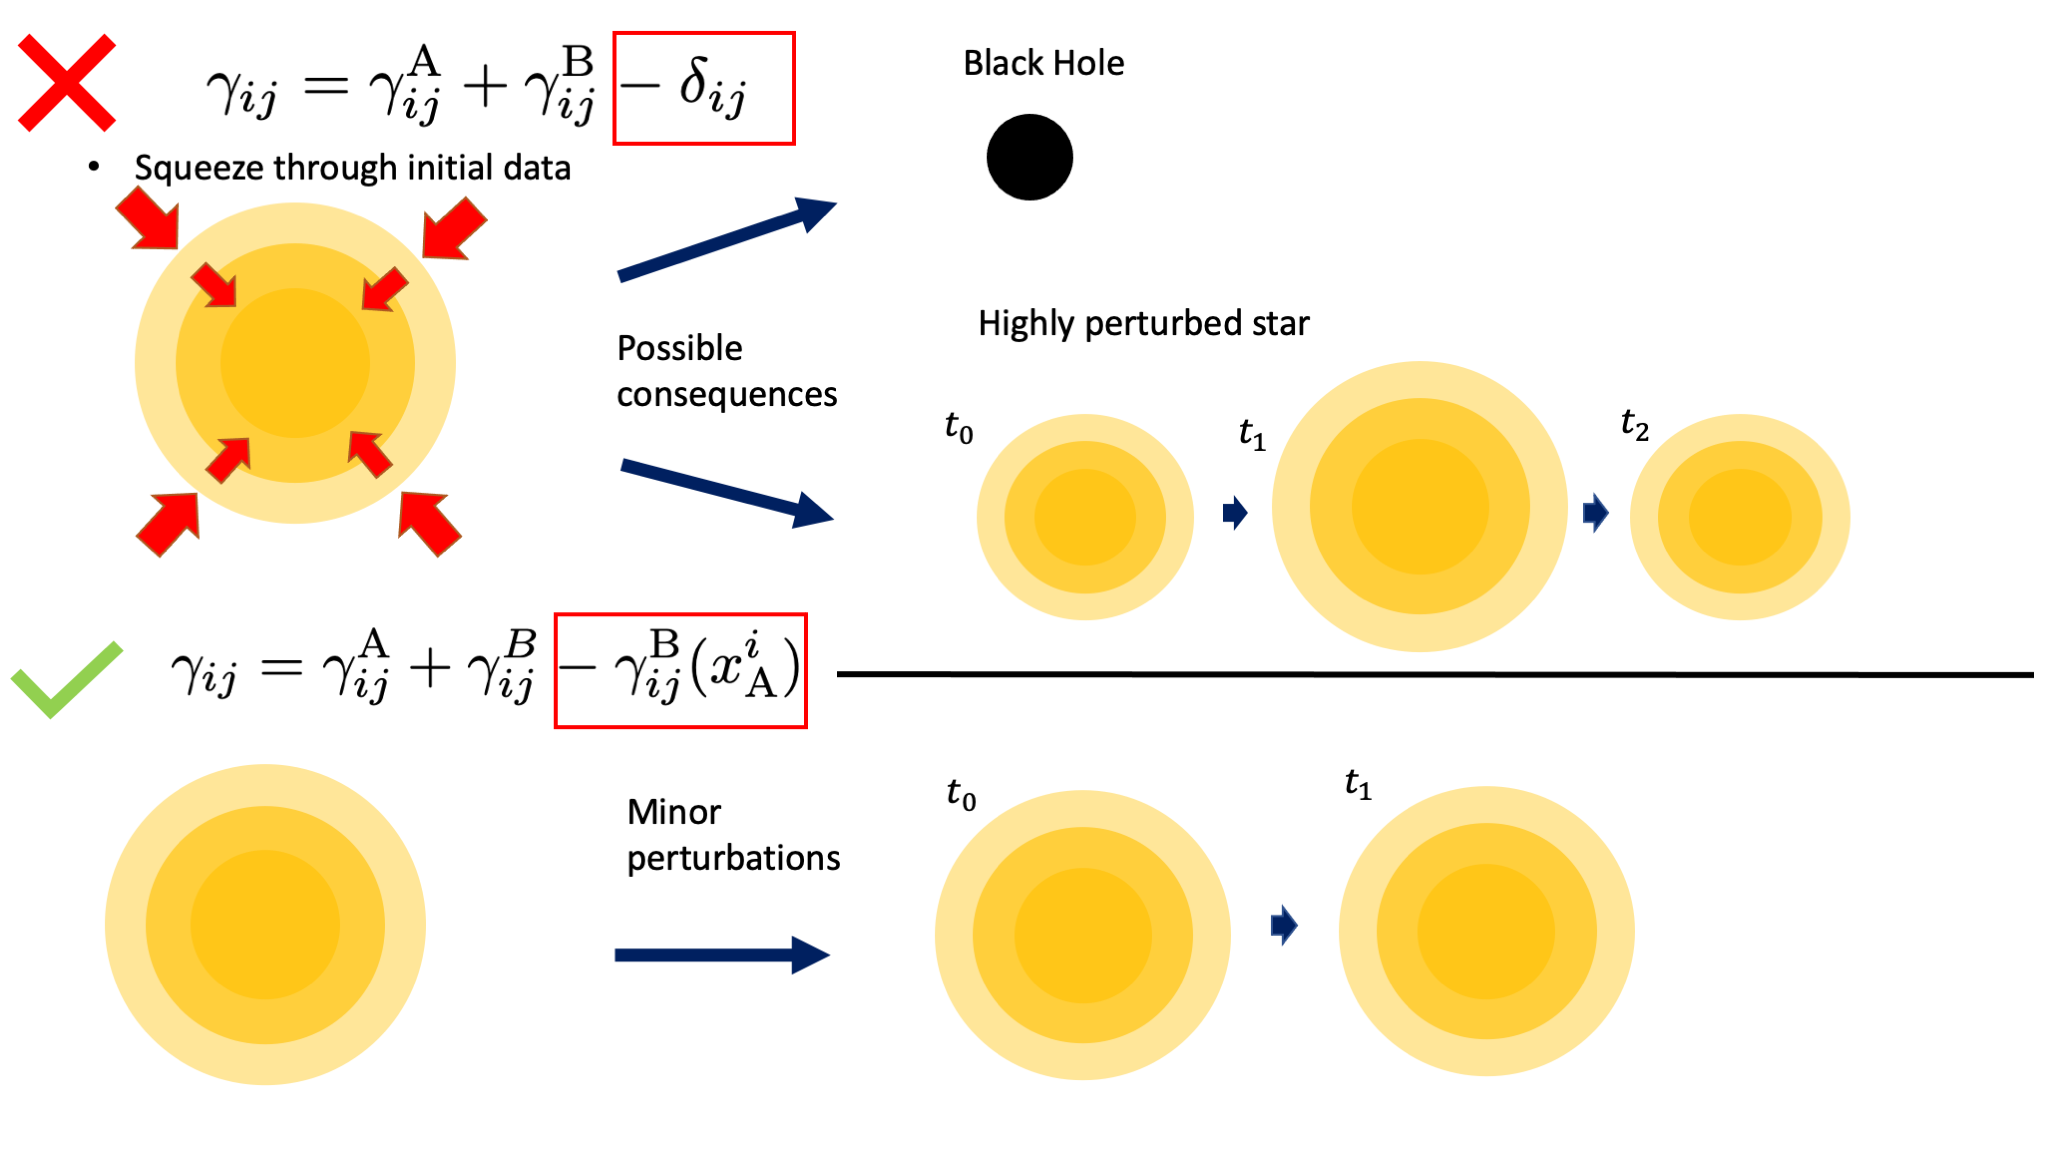
\includegraphics[width=350pt]{BosonStarTrick.png}
    \caption{
    Graphical illustration of the spurious dynamics that
    may be introduced by the simple superposition
    procedure (\ref{eq:superpossimple}). {\it Upper panel}:
    The spurious
    increase in the volume element mimics a squeezing of the
    stellar core that effects a pulsation of the star or
    may even trigger gravitational collapse to a BH.
    {\it Lower panel}: No such squeezing occurs with the
    adjusted superposition (\ref{eq:superposplus}),
    and the binary evolution starts with approximately
    unperturbed stars.
    }
    \label{fig:Overview}
\end{figure}
%
Fig.~\ref{fig:Overview} together with some of the possible
consequences.
As we will see, this qualitative interpretation is fully borne out
by the phenomenology we observe in the binaries' time evolutions.

Finally, we would like to emphasise that, while evaluating the constraint violations is in general a good rule of thumb to check whether the field configuration is a solution of the system, it does \emph{not} inform one whether it is \emph{the intended} solution; a system with some constraint violation may have drifted closer to a different, unintended solution. In the present case, in addition to the  increased constraint violation, the constructed BS solutions possess significant excitations. Thus, while applying a constraint damping system like conformal Z4
\cite{Bernuzzi:2009ex,Alic:2011gg}
may eventually drive the system to a solution, it may no longer be what was originally intended to be the initial condition of an unexcited BS star.


%=============================================================================
\subsection{Improved superposition}
%
The problem of the simple superposition is encapsulated
by Eq.~(\ref{eq:metricpert}) and the resulting deviation
of the volume elements at the stars' centres away from their
equilibrium values. At the same time, the equation presents us
with a concrete recipe to mitigate this error: we merely need
to replace in the simple superposition (\ref{eq:superpossimple})
the first relation $\gamma_{ij}=\gamma_{ij}^{\rm A}+\gamma_{ij}^B
-\delta_{ij}$ by
%
\begin{equation}
  \boxed{
  \gamma_{ij}=\gamma_{ij}^{\rm A}+\gamma_{ij}^{\rm B}
  -\gamma_{ij}^{\rm B}(x^i_{\rm A})
  =\gamma_{ij}^{\rm A}+\gamma_{ij}^{\rm B}
  -\gamma_{ij}^{\rm A}(x^i_{\rm B})\,.}
  \label{eq:superposplus}
\end{equation}
%
The two expressions on the right-hand side are indeed equal thanks
to the symmetry of our binary: its constituents have equal mass,
no spin and their velocity components satisfy
$v_{\rm A}^i v_{\rm A}^j=v_{\rm B}^i v_{\rm B}^j$ for all
$i,\,j=1,\,2,\,3$ in the centre-of-mass frame.
Equation (\ref{eq:superposplus}) manifestly ensures that at
positions $x_{\rm A}^i$ and $x_{\rm B}^i$ we now recover
the respective star's equilibrium metric and, hence, volume element.
We graphically illustrate this improvement in the bottom panel
of Fig.~\ref{fig:Overview}.

A minor complication arises from the fact that the resulting
spatial metric does not asymptote towards $\delta_{ij}$
as $R\rightarrow \infty$. We accordingly impose
outgoing Sommerfeld boundary conditions on the asymptotic
background metric $2\delta_{ij}-\gamma_{ij}^{\rm A}(x^i_{\rm B})$;
in a set of test runs, however, we find this correction to result
in very small changes well below the simulation's discretisation errors.

Finally, we note that the leading-order correction to the superposition
as written in Eq.~(\ref{eq:superposplus}) does not work for asymmetric
configurations with unequal masses or spins. Generalising the method
to arbitrary binaries requires the subtraction of 
a spatially varying term rather than a constant
$\gamma_{ij}^{\rm B}(x^i_{\rm A})=\gamma_{ij}^{\rm A}(x^i_{\rm B})$
or $\delta_{ij}$. Such a generalisation may consist, for example,
of a weighted sum of the terms $\gamma_{ij}^{\rm A}(x^i_{\rm B})$
and $\gamma_{ij}^{\rm B}(x^i_{\rm A})$. Leaving this
generalisation for future work, we will focus on equal-mass
systems in the remainder of this study and explore
the degree of improvement achieved with
Eq.~(\ref{eq:superposplus}).

%\el{We should also mention that since the effect scales as $\sqrt{r}$, increasing the distance of the initial separation \emph{may} not help as much, and may increase other inaccuracies associated with a long infall evolution. The argument for $\sqrt{r}$ is described in the \cite{Helfer:2018vtq}, i.e. using a Schwarzchild ansatz, the determinant scales like $\sqrt{r}$ for small perturbations.}

%=============================================================================
\section{Models and results}
\label{sec:results}
%
For our analysis of the two types of superposed initial data,
we will now discuss time evolutions of binary BS head-on collisions.
A head-on collision is characterised
by the two individual BS models and three further parameters,
the initial separation in units of the ADM mass,
$d/M$,
%\mr{Worth defining $M$ here?}
%\us{I thought I had defined it, but maybe I didn't. Might be
%worth redefining anyway. Done.}
and the initial velocities $v_{\rm A}$ and
$v_{\rm B}$ of the BSs. We perform all our simulations in the centre-of-mass
frame, so that for equal-mass binaries, $v_{\rm A}=-v_{\rm B}\invdefeq v$.
One additional parameter arises from the type of superposition
used for the initial data construction: we either use the
``plain'' superposition of Eq.~(\ref{eq:superpossimple}) or
the ``adjusted'' method (\ref{eq:superposplus}).

For all our simulations, we
set $v=0.1$; this value
allows us to cover a wide range of initial separations 
without the simulations becoming prohibitively long.
%
\begin{table}[t]
    \centering
    \caption{The four types of BS binary head-on collisions simulated
    in this study. The individual BSs A and B are given either
    by the mini or solitonic model of Table \ref{tab:models},
    and start with initial
    velocity $v$ directed towards each other. The initial data
    is constructed either by plain superposition
    (\ref{eq:superpossimple}) or by adjusting
    the superposed data according to Eq.~(\ref{eq:superposplus}).
    %Appendix A in Ref.~\cite{Helfer:2018vtq}.
    For each type of binary, we perform five collisions with
    initial separations $d$ listed in the final column.
    %\us{For my own use: The convergence sequences are
    %{\tt mBShod080\_h,~~tmBShod080\_h,~~lsBShod16\_h,~~tlsBShod%16\_h.}}
    }
    \begin{tabular}{r|ccccc}
    \hline
    Label & star A & star B & $v$ & initial data & $d/M$ \\
    \hline
    {\tt mini} & mini & mini & $0.1$ & plain &
    75.5,~101,~126,~151,~176 \\
    {\tt +mini}& mini & mini & $0.1$ & adjusted &
    75.5,~101,~126,~151,~176 \\
    {\tt soli} & soli & soli & $0.1$ & plain &
    16.7,~22.3,~27.9,~33.5,~39.1 \\
    {\tt +soli} & soli & soli & $0.1$ &
    adjusted &
    16.7,~22.3,~27.9,~33.5,~39.1 \\
    \hline
    \end{tabular}
    \label{tab:hods}
\end{table}
%
The BS binary configurations
summarised in Table \ref{tab:hods} then result
in four sequences of head-on collisions labelled
{\tt mini}, {\tt +mini}, {\tt soli} and {\tt +soli},
depending in the nature of the constituent BSs and
the superposition method. For each sequence, we vary the
BSs initial separation $d$ to estimate the dependence of the
outcome on $d$. First, however, we test our interpretation
of the improved superposition (\ref{eq:superposplus})
by computing the level of constraint violations in the
initial data.
%%
%\begin{table}[ht]
%    \centering
%    \begin{tabular}{r|ccccc}
%    \hline
%    Label & BS 1 & BS 2 & $v$ & initial data & initial grid \\
%    \hline
%    {\tt mini} & mini & mini & $0.1$ & plain &
%    $\{(645,322,161)\times(40,20,10),\,h\}$ \\
%    {\tt +mini}& mini & mini & $0.1$ & adjusted &
%    $\{(645,322,161)\times(40,20,10)$,\,h\} \\
%    {\tt soli} & soli & soli & $0.1$ & plain &
%    $\{(357,179,89,45)\times(5.6,2.8,1.4),\,h\}$ \\
%    {\tt +soli} & soli & soli & $0.1$ &
%    adjusted &
%    $\{(357,179,89,45)\times(5.6,2.8,1.4),\,h\}$ \\
%    \hline
%    \end{tabular}
%    \caption{The four types of BS binary head-on %collisions simulated
%    in this study. The individual BSs 1 and 2 are %given either
%    by the mini or solitonic model of Table \ref{tab:models},
%    and start with initial
%    velocity $v$ directed towards each other. The initial data
%    is constructed either by plain superposition
%    (\ref{eq:superpossimple} or by adjusting
%    the superposed data according to Eq.~(\ref{eq:superposplus}).
%    %Appendix A in Ref.~\cite{Helfer:2018vtq}.
%    The initial grid setup consists
%    of $N_1$ nested boxes centered on the origin and $N_2$
%    pairs of boxes centered around one boson star center,
%    respecitvely. The half widths of the boxes are specified
%    as $(r_1,\ldots,r_{N_1})\times(r_{N_1+1},\ldots,r_{N_1+N_2})$.
%    The grid spacing is $h$ in the innermost levels and increases
%    by a factor 2 consecutively on each outer refinement level.
%    Within each type of collisions, we vary the initial separation of the boson stars as listed in
%    Table \ref{tab:results}. Label: {\tt tab:hods}
%    %\us{For my own use: The convergence sequences are
%    %{\tt mBShod080\_h,~~tmBShod080\_h,~~lsBShod16\_h,~~tlsBShod%16\_h.}}
%    }
%    \label{tab:hods}
%\end{table}
%%

%The set of head-on collisions simulated in this work is given in
%Table \ref{tab:hods}. A further parameter arises from the
%construction of the initial data by either superposing the
%individual BS spacetimes according to Eq.~(??) or by correcting
%the volume element according to the method of Appendix A of
%Ref.~\cite{Helfer:2018vtq}.





%%
%\begin{table}
%    \centering
%    \begin{tabular}{l|cccccc}
%    \hline
%    Model & $\sqrt{G}A_{\rm ctr}$ & $\sqrt{G}\sigma_0$ & $\mu M_{\rm BS}$ & $\omega/\mu$ & $\mu R_{90}$ & $\max\frac{m(r)}{r}$  \\
%    \hline
%    mini & 0.0124 & $\infty$ & $0.395$ & $0.971$ & $15.24$ & $0.0249$ \\
%    soli & 0.17 & $0.2$ & $0.713$ & $0.439$ & $2.93$ & $0.222$ \\
%    \hline
%    \end{tabular}
%    \caption{Parameters of the two single, spherically symmetric
%    ground state boson star models employed for our simulations of
%    head-on collisions. Up to the rescaling with the scalar mass
%    $\mu$, each boson star is determined by the central amplitude
%    $A_{\rm ctr}$ of the scalar field and the potential parameter
%    $\sigma_0$ of Eq.~(\ref{eq:pot}). The mass $M_{\rm BS}$ of the boson star,
%    the scalar field frequency $\omega$, the radius $R_{90}$ containing
%    $90\,\%$ of the total mass $M_{\rm BS}$ and the compactness, defined here
%    as the maximal ratio of the mass function to radius, represent
%    the main features of the stellar model.}
%    \label{tab:models}
%\end{table}
%%
%by the two individual BS models and three further parameters,
%the initial separation $d/M$ and the initial velocities $v_1$ and
%$v_2$ of the BSs. We perform all out simulations in the center-of-mass
%frame, so that for equal-mass binaries, $v_1=-v_2\invdefeq v$.
%The set of head-on collisions simulated in this work is given in
%Table \ref{tab:hods}. A further parameter arises from the
%construction of the initial data by either superposing the
%individual BS spacetimes according to Eq.~(??) or by correcting
%the volume element according to the method of Appendix A of
%Ref.~\cite{Helfer:2018vtq}.

%=============================================================================
\subsection{Initial constraint violations}
%
As discussed in Sec.~\ref{sec:superpossimple} and in Appendix
A of Ref.~\cite{Helfer:2018vtq},
the main shortcoming of the plain superposition procedure
consists in the distortion of the volume element near the
individual BSs' centres and the resulting perturbation
of the mass-energy inside the stars away from their equilibrium
values. If this interpretation is correct, we would expect
this effect to manifest itself in an elevated level of violation
of the Hamiltonian constraint
(\ref{eq:ham}) which relates the energy density to the
spacetime curvature. Put the other way round, we would
expect our improved method (\ref{eq:superposplus}) to reduce the
Hamiltonian constraint violation. This is indeed the case
as demonstrated in the upper panels of
Fig.~\ref{fig:ham} where we plot the
Hamiltonian constraint violation of the initial data
along the collision axis for the configurations
{\tt mini} and {\tt +mini} with $d=101\,M$ and 
the configurations {\tt soli} and {\tt +soli} with
$d=22.3\,M$.
%
\begin{figure}
  \centering
  \includegraphics[width=300pt]{constraints.eps}
  \caption{Upper row: The Hamiltonian constraint violation $\mathcal{H}$ --
  Eq.~(\ref{eq:ham}) -- normalised by the respective BS's
  central energy density $16\pi \rho_{\rm ctr}$
  is plotted along the collision
  axis of the binary configurations {\tt mini}, {\tt +mini}
  with $d=101\,M$ (left) and {\tt soli}, {\tt +soli} with $d=22.3\,M$ (right).
  The degree of violations is substantially reduced in the
  BS interior by using
  the improved superposition (\ref{eq:superposplus})
  for {\tt +mini} and {\tt +soli} relative to their plain
  counterparts; the maxima of $\mathcal{H}$ have dropped by
  over an order of magnitude in both cases.
  Bottom row: The same analysis for the momentum constraint
  $\mathcal{M}_x$
  normalised by the central BS's momentum density
  $8\pi j_x$. Here the improvement is less dramatic,
  but still yields a reduction by a factor of a few
  in the BS core.
  }
  \label{fig:ham}
\end{figure}
%

In the limit of zero boost velocity $v=0$, this effect is even
tractable through an analytic calculation which confirms
that the improved superposition (\ref{eq:superposplus})
ensures $\mathcal{H}=0$ at the BS's centres in isotropic
coordinate; see \ref{sec:hamanalytic} for more details.

Our adjustment (\ref{eq:superposplus}) also leads to
a reduction of the momentum constraint violations of the
initial data, although the effect is less dramatic here.
The bottom panels of Fig.~\ref{fig:ham} display the
momentum constraint $\mathcal{M}_x$ of Eq.~(\ref{eq:mom})
along the collision axis normalised by the momentum
density $8\pi j_x$; we see a reduction by a factor of a few
over large parts of the BS interior for the modified
data {\tt +mini} and {\tt +soli}.

The overall degree of initial constraint violations is
rather small in all cases, well below $0.1\,\%$ for
our adjusted data. These data should therefore also
provide a significantly improved initial guess for
a full constraint solving procedure. We leave such an
analysis for future work and in the remainder of the
work explore the impact of the adjustment
(\ref{eq:superposplus}) on the physical results
obtained from the initial data's time evolutions.

%=============================================================================
\subsection{Convergence and numerical uncertainties}
%
In order to put any differences in the time evolutions
into context, we need to understand the uncertainties
inherent to our numerical simulations. For this purpose,
we have studied the convergence of the GW radiation
generated by the head-on collisions of mini and solitonic
BSs.
%with $d=101\,M$ and $d=22.3\,M$, respectively.

Figure \ref{fig:conv_tmBS_Erad} displays the convergence
of the radiated energy $E_{\rm rad}$ as a function
of time for the {\tt +mini} configuration with $d=101\,M$ of
Table \ref{tab:models} obtained for grid resolutions
$h_1=M/6.35$, $h_2=M/9.53$ and $h_3=M/12.70$ on the
innermost refinement level and corresponding grid 
spacings on the other levels. The functions
$E_{\rm rad}(t)$ and their differences are shown in the
bottom and top panel, respectively, of Fig.~\ref{fig:conv_tmBS_Erad}
together with an amplification of the high-resolution
differences by the factor $Q_2=2.86$ for second-order
convergence. The observation of second-order convergence
is compatible with the second-order ingredients of the
{\sc Lean} code, prolongation in time and the outgoing
radiation boundary conditions. We believe that this
dominance is mainly due to the smooth behaviour
of the BS centre as compared with the case of black holes
\cite{Husa:2007hp}. By using the second-order
Richardson extrapolated result, we determine the
discretisation error of our energy estimates as
$0.9\,\%$ for $h_3$ which is the resolution employed
for all remaining mini BS collisions. We have performed
the same convergence analysis for the plain-superposition
counterpart {\tt mini} and for the dominant $(\ell,m)=(2,0)$
multipole of the Newman-Penrose scalar of both configurations
and obtained the same convergence and very similar relative
errors.
%
%\begin{figure}
%    \centering
%    \includegraphics[width=250pt]{conv_mBS_psi20.eps}
%    \caption{Convergence analysis of the $(\ell,m)=(2,0)$ multipole
%    of $\Psi_4$ extracted at $r=200$ from the collision
%    {\tt mBS\_hod080} using resolutions $h_1=1/8$, $h_2=1/12$
%    and $h_3=1/16$. The dotted line represents the
%    second-order Richardson extrapolation. In the top panel, the difference between
%    the higher-resolution results has been amplified by
%    $Q_2=2.857$ corresponding to second-order convergence.
%    \us{Convert to correct units involving the mass and add
%    table of our set of runs.} For reference, we show in the
%    bottom panel
%    the $(2,0)$ multiple obtained at high resolution.
%    Label: {\tt fig:conv\_mBS\_psi20}}
%    \label{fig:conv_mBS_psi20}
%\end{figure}
%
%\begin{figure}
%    \centering
%    \includegraphics[width=250pt]{conv_mBS_Erad.eps}
%    \caption{Convergence analysis for gravitational-wave
%    energy extracted at $R_{\rm ex}=200$
%    from the head-on collision {\tt mBShod100} of Table
%    \ref{tab:hods}. For the resolutions
%    $h_1=1/8$, $h_2=1/12$ and $h_3=1/16$, we obtain convergence
%    close to second order (upper panel). The numerical error,
%    obtained by comparing our results
%    with the second-order Richardson extrapolated values
%    (bottom panel), is $0.8\,\%$ ($1.5\,\%$, $3.3\,\%$) for
%    our high (medium, coarse) resolutions.
%    Label: {\tt fig:conv\_mBS\_Erad}}
%    \label{fig:conv_mBS_Erad}
%\end{figure}
%%

In Fig.~\ref{fig:conv_tsBS_Erad}, we show the same
convergence analysis for the solitonic collision
{\tt +soli} with $d=22.3\,M$ and resolutions
$h_1=M/22.9$, $h_2=M/45.9$, $h_3=M/68.8$. We observe
second-order convergence during merger and ringdown and
slightly higher convergence in the earlier infall phase.
%
\begin{figure}[t]
    \centering
    \includegraphics[width=250pt]{conv_tmBS_Erad.eps}
    \caption{
    Convergence analysis for the GW energy extracted at
    $R_{\rm ex}=252\,M$ from the head-on collision
    {\tt +mini} of Table \ref{tab:models} with
    $d=101\,M$. For the resolutions
    $h_1=M/6.35$, $h_2=M/9.53$ and $h_3=12.70$
    (on the innermost refinement level),
    we obtain convergence close to second order
    (upper panel). The numerical error,
    obtained by comparing our results
    with the second-order Richardson extrapolated values
    (bottom panel), is $0.9\,\%$ ($1.6\,\%$, $3.6\,\%$) for
    our high (medium, coarse) resolutions.
    %Label: {\tt fig:conv\_tmBS\_Erad}
    }
    \label{fig:conv_tmBS_Erad}
\end{figure}
%
%
\begin{figure}[t]
    \centering
    \includegraphics[width=250pt]{conv_tsBS_Erad.eps}
    \caption{Convergence analysis as in
    Fig.~\ref{fig:conv_tmBS_Erad} but for the configuration
    {\tt +soli} of Table \ref{tab:models} with
    $d=22.3\,M$ and
    resolutions $h_1=M/22.9$, $h_2=M/45.9$ and $h_3=M/68.8$.
    The numerical error,
    obtained by comparing our results
    with the second-order Richardson extrapolated values
    (bottom panel),
    %is $0.02\,\%$ ($0.04\,\%$, $0.2\,\%$) for
    is $0.03\,\%$ ($0.07\,\%$, $0.6\,\%$) for
    our high (medium, coarse) resolutions.
    %Label: {\tt fig:conv\_tsBS\_Erad}
    }
    \label{fig:conv_tsBS_Erad}
\end{figure}
%
For the uncertainty estimate we conservatively use
the second-order Richardson extrapolated result and
obtain a discretisation error of about $0.07\,\%$ for
our medium resolution $h_2$ which is the value
we employ in our solitonic production runs. Again,
we have repeated this analysis for the plain
{\tt soli} counterpart and the $(2,0)$ GW multipole
observing the same order of convergence and similar uncertainties. Our error estimate for the solitonic
configurations is rather small in comparison to the
mini BS collisions and we cannot entirely rule out a
fortuitous cancellation of errors in our simulations.
From this point on, we therefore use a conservative
discretisation error estimate of $1\,\%$ for all
our BS simulations.


A second source of uncertainty in our results is due
to the extraction of the GW signal at finite radii
rather than $\mathcal{I}^+$. We determine this error
by extracting the signal at multiple radii, fitting
the resulting data by the series expansion
$f=f_0+f_1/r$, and comparing the result at our outermost
extraction radius with the limit $f_0$. This procedure
results in errors in $E_{\rm rad}$ ranging between $0.5\,\%$
and $3\,\%$. With the upper range, we arrive at
a conservative total error budget for discretisation and
extraction of about $4\,\%$.
As a final test, we have repeated the {\tt mini} and
{\tt +mini} collisions for $d=101\,M$
with the independent {\sc GRChombo}
code \cite{Clough:2015sqa,Radia:2021} using the CCZ4 formulation \cite{Alic:2011gg} and obtain the same results within $\approx 1.5\,\%$.
Bearing in mind these tests and a $4\,\%$ error budget,
we next study the dynamics of the BS head-on collisions
with and without our adjustment of the initial data.
%%
%\begin{figure}
%    \centering
%    \includegraphics[width=250pt]{conv_sBS_Erad.eps}
%    \caption{Convergence analysis as in
%    Fig.~\ref{fig:conv_tmBS_Erad} but for the configuration
%    {\tt sBS\_hod022} of Table \ref{tab:hods} and using
%    resolutions $h_1=1/16$, $h_2=1/32$ and $h_3=1/48$.
%    The numerical error,
%    obtained by comparing our results
%    with the third-order Richardson extrapolated values
%    (bottom panel), is $0.03\,\%$ ($0.07\,\%$, $0.6\,\%$) for
%    our high (medium, coarse) resolutions.
%    Label: {\tt fig:conv\_sBS\_Erad}
%    }
%    \label{fig:conv_sBS_Erad}
%\end{figure}
%%


%=============================================================================
\subsection{Radiated gravitational-wave energy}
%
For our first test, we compute the total radiated
GW energy for all our head-on collisions focusing
in particular on its dependence on the initial separation
$d$ of the BS centres. In this estimate we exclude
any spurious or ``junk'' radiation content
of the initial data by starting the integration
at $t=R_{\rm ex}+40\,M$. Unless specified otherwise,
all our results are extracted at $R_{\rm ex}=300\,M$ for
mini BS collisions and $R_{\rm ex}=84\,M$ for the
solitonic binaries.
%
\begin{figure}
    \centering
    \includegraphics[width=250pt]{erad.eps}
    \caption{The GW energy $E_{\rm rad}$ generated in
    the head-on collision of mini (upper panel) and solitonic (lower panel) BS binaries starting
    with initial separation $d$ and velocity $v=0.1$ towards
    each other.
    For comparison, a non-spinning, equal-mass BH binary
    colliding head-on with the same boost velocity $v=0.1$ radiates $E_{\rm rad}=6.0\times 10^{-4}\,M$
    \cite{Sperhake:2019oaw}.
    %Label: {\tt fig:erad}
    } 
    \label{fig:erad}
\end{figure}
%

The main effect of increasing the initial separation is a
reduction of the (negative) binding energy of the binary and a corresponding
increase of the collision velocity around merger. In the large
$d$ limit, however, this effect becomes negligible. For the
comparatively large initial separations chosen in our
collisions, we would therefore
expect the function $E_{\rm rad}$ to be approximately constant,
possibly showing a mild increase with $d$. The mini BS collisions
shown as black $\times$ symbols in the upper panel of
Fig.~\ref{fig:erad} exhibit a rather different behaviour:
the radiated energy rapidly decreases with $d$ and only levels
off for $d\gtrsim 150\,M$. We have verified that the excess
energy for smaller $d$ is not due to an elevated level of
junk radiation which consistently contribute well below 
%\mr{Change to \%?} \us{Not sure this will look better... Is
%$0.1\,\%$ an improvement over $10^{-3}$?}
$0.1\,\%$ of $E_{\rm rad}$ in all our mini BS collisions and has
been excluded from the results of Fig.~\ref{fig:erad} anyway.
The {\tt +mini} BS collisions,
in contrast, results in an approximately constant $E_{\rm rad}$
with a total variation approximately at the level of the
numerical uncertainties. For $d\gtrsim 150\,M$, both types of
initial data yield compatible results, as is expected.
The key benefit of our adjusted initial data is that they provide
reliable results even for smaller initial separations suitable
for starting BS inspirals.

The discrepancy is less pronounced for the head-on collisions
of solitonic BS collisions; both types of initial data result
in approximately constant $E_{\rm rad}$. They differ, however,
in the predicted amount of radiation at a level that
is significant compared to
the numerical uncertainties. As we will see below, this difference
is accompanied by drastic differences in the BS's dynamics during the
long infall period. We furthermore note that the mild but
steady increase obtained for the adjusted {\tt +soli} agrees
better with the physical expectations.

The differences in the total radiated GW energy also manifest themselves
in different amplitudes of the $(2,0)$ multipole of the Newman-Penrose
scalar $\Psi_4$. This is displayed in Figs.~\ref{fig:mini_psi20}
and \ref{fig:soli_psi20} where we show the GW modes for the mini and
solitonic collisions, respectively. The most prominent difference
between the results for plain and adjusted initial data is the
significant variation of the amplitude of the $(2,0)$ mode in the
plain mini BS collisions in the upper panel of Fig.~\ref{fig:mini_psi20}.
In contrast, the differences in the amplitudes in Fig.~\ref{fig:soli_psi20}
for the solitonic collisions are very small. In fact, the differences
in the radiated energy of the {\tt soli} and {\tt +soli} collisions mostly
arise from a minor stretching of the signal for the {\tt soli} case; this
effect is barely perceptible in Fig.~\ref{fig:soli_psi20} but is amplified
by the integration in time when we calculate the energy. Finally, we note
the different times of arrival of the main pulses in Fig.~\ref{fig:soli_psi20};
especially for larger initial separation, the merger occurs earlier for
the {\tt soli} configurations than for their adjusted counterparts
{\tt +soli}.
We will discuss this effect together with the evolution
of the scalar field amplitude in the next subsection.
%\us{Do we wish to keep these two figures and the discussion? Let's gather our thoughts...}
% \mr{I'm in favour of keeping it. 
% Are you just concerned that you have too many figures? If so,
% I would be inclined to drop a convergence figure 
% (e.g. Fig.~\ref{fig:conv_tmBS_Erad}).}
% \us{It was not so much the number of figures but whether the
% waveforms told us anything beyond the total radiated energy.
% Initially I was convinced that they did not, but when I added
% the discussion about the different arrival times, I wasn't so
% sure and also inclined more towards keeping them...}
%\us{Add GRChombo simulations somewhere; gotta read the whole thing to
%find the best place...}
%\us{We might drop these two figures; and merely keep one sentence saying
%that ``the observed dependence of the radiated GW energy on the type
%of initial data and/or the initial separation is mirrored by corresponding
%differences in the amplitudes of the $(2,0)$ multipole of the Newman-Penrose
%scalar $\Psi_4$.'' Let me know your thoughts.}



%%
%\begin{table}[]
%    \centering
%    \begin{tabular}{r|cc}
%      \hline
%      Label & $d/M$ & $E_{\rm rad}/M$ \\
%      \hline
%      {\tt mini} & 75.5 & $9.78\times 10^{-5}$
%      \\
%      {\tt mini} & 101 & $8.39\times 10^{-5}$
%      \\
%      {\tt mini} & 126 & $7.39\times 10^{-5}$
%      \\
%      {\tt mini} & 151 & $6.84\times 10^{-5}$
%      \\
%      {\tt mini} & 176 & $6.88\times 10^{-5}$
%      \\
%      \hline
%      {\tt +mini} & 75.5 & $7.14 \times 10^{-5}$
%      \\
%      {\tt +mini} & 101 & $6.83\times 10^{-5}$
%      \\
%      {\tt +mini} & 126 & $6.72\times 10^{-5}$
%      \\
%      {\tt +mini} & 151 & $6.63\times 10^{-5}$
%      \\
%      {\tt +mini} & 176 & $6.67\times 10^{-5}$
%      \\
%      \hline
%    \end{tabular}
%    %
%    \hspace{0.5cm}
%    \begin{tabular}{r|ccc}
%      \hline
%      Label & $d/M$ & $E_{\rm rad}/M$ & $(t_{\rm peak}-t_{\rm AH})/M$ \\
%      \hline
%      {\tt soli} & 16.7 & $7.34\times 10^{-4}$ & 126.3
%      \\
%      {\tt soli} & 22.3 & $7.21\times 10^{-4}$ & 139.9
%      \\
%      {\tt soli} & 27.9 & $7.15\times 10^{-4}$ & 152.4
%      \\
%      {\tt soli} & 33.5 & $7.18\times 10^{-5}$ & 164.1
%      \\
%      {\tt soli} & 39.1 & $7.32\times 10^{-5}$ & 172.0
%      \\
%      \hline
%      {\tt +soli} & 16.7 & $6.17 \times 10^{-4}$ & 93.5
%      \\
%      {\tt +soli} & 22.3 & $6.28\times 10^{-4}$ & 94.7
%      \\
%      {\tt +soli} & 27.9 & $6.36\times 10^{-4}$ & 95.8
%      \\
%      {\tt +soli} & 33.5 & $6.43\times 10^{-4}$ & 96.1
%      \\
%      {\tt +soli} & 39.1 & $6.50\times 10^{-4}$ & 96.5
%      \\
%      \hline
%    \end{tabular}
%    \caption{Results from the sequences of boson star collisions

%   with initial separation $d$. $E_{\rm rad}$ denotes the
%    energy radiated in gravitational waves, $u_{\rm mer}$ is
%    the (retarded) time of the maximal GW amplitude of $\psi_{20}$
%    and $u_{\rm AH}$ the retarded time of the first formation
%    of an apparent horizon. For mini boson star collisions, no
%    apparent horizons form and we leave the latter entry empty.
%    For comparison, a non-spinning, equal-mass BH binary
%    colliding head-on with the same boost velocity $v=0.1$ radiates $E_{\rm rad}=6.0\times 10^{-4}\,M$
%    \cite{Sperhake:2019oaw}.
%    Label: {\tt tab:results}
%    }
%    \label{tab:results}
%\end{table}
%
%
\begin{figure}
    \centering
    \includegraphics[width=250pt]{mini_psi20.eps}
    \caption{The $(2,0)$ mode of the Newman-Penrose scalar
    for the mini boson star collisions of Table \ref{tab:models}.
    %Label: {\tt fig:mini\_psi20}
    }
    \label{fig:mini_psi20}
\end{figure}
%
%
\begin{figure}
    \centering
    \includegraphics[width=250pt]{soli_psi20.eps}
    \caption{The $(2,0)$ mode of the Newman-Penrose scalar
    for the solitonic boson star collisions of Table \ref{tab:models}.
    %Label: {\tt fig:soli\_psi20}
    }
    \label{fig:soli_psi20}
\end{figure}
%

%=============================================================================
\subsection{Evolution of the scalar amplitude and gravitational collapse}
%
The adjustment (\ref{eq:superposplus}) in the superposition of oscillatons
was originally developed in Ref.~\cite{Helfer:2018vtq} to reduce
spurious modulations in the scalar field amplitude; cf.~their
Fig.~7. In our simulations, this effect manifests itself
most dramatically in the collisions of our solitonic BS
configurations {\tt soli} and {\tt +soli}.
From Fig.~\ref{fig:statBS}, we recall that the single-BS constituents
of these binaries are stable, but highly compact stars, located
fairly close to the instability threshold. We would therefore expect
them to be more sensitive to spurious modulations in their central
energy density. This is exactly what we observe in all time evolutions
of the {\tt soli} configurations starting with plain-superposition
initial data. As one example, we show
in Fig.~\ref{fig:soli_ampctr} the scalar amplitude
at the individual BS centres and the BS trajectories
as functions of time for the
{\tt soli} and {\tt +soli} configurations starting with initial
separation $d=22.3\,M$.
%
\begin{figure}
    \centering
    \includegraphics[width=250pt]{ampctr_sBS.eps}
    \caption{The central scalar-field amplitude $|\varphi_{\rm ctr}|$ 
    as a function of time for one BS in the head-on
    collisions of solitonic BSs with distance $d=22.3\,M$
    (black solid and red long-dashed) as well as a single
    BS spacetime with the same parameters (green dashed)
    and the same single BS spacetime ``poisoned'' with
    the metric perturbation (\ref{eq:metricpert}) that would arise in a simple
    superposition (see text for details). The dotted
    vertical lines mark the first location of an
    apparent horizon in the simulation of the same colour;
    as expected, no horizon ever forms in the evolution
    of the unpoisoned single BS.
    In the bottom panel, we show for reference the coordinate
    trajectories of the BS centres as obtained from locally
    Gauss-fitting the scalar profile. Around merger this procedure
    becomes inaccurate, so that the values around $t\approx 70\,M$
    should be regarded as qualitative measures, only.
    %Label: {\tt fig:soli\_ampctr}
    }
    \label{fig:soli_ampctr}
\end{figure}
%
Let us first consider the {\tt soli} configuration using plain
superposition displayed by the solid (black) curves. In the upper
panel of Fig.~\ref{fig:soli_ampctr}, we clearly see
that the scalar amplitude steadily increases, reaching a maximum
around $t\approx 30\,M$ and then rapidly drops to a near-zero level.
Our interpretation of this behaviour as a collapse to a BH is confirmed
by the horizon finder which reports an apparent horizon of irreducible
mass $m_{\rm irr}=0.5\,M$ just before the scalar field amplitude
collapses; the time of the first identification of an apparent horizon
is marked by the vertical dotted black line at $t\approx 30\,M$.
For reference we plot in the bottom panel the trajectory of the BS centres
along their collision (here the $x$) axis. In agreement with the
horizon mass $m_{\rm irr}=0.5\,M$, the trajectory clearly indicates
that around $t\approx 30\,M$, the BSs are still far away from merging
into a single BH; in units of the ADM mass,
the individual BS radius is $r_{99}=2.78\,M$. We interpret
this early BH collapse as a spurious feature due to the use of
plain superposition in the initial data construction.
This behaviour is also seen in the case of the real scalar
field oscillatons in \cite{Helfer:2018vtq}.

We have tested this hypothesis with the evolution
of the adjusted initial data.
These exhibit a drastically different behaviour
in the collision {\tt +soli} displayed by the dashed (red) curves in
Fig.~\ref{fig:soli_ampctr}.
Throughout most of the infall, the central scalar amplitude
is constant, it increases mildly when the BS trajectories meet near $x=0$,
and then rapidly drops to zero. Just as the maximum amplitude is reached,
the horizon finder first computes an apparent horizon, now with 
%\mr{In terms of $M$?} \us{Oh yes! Fixed.}
$m_{\rm irr}=0.99\,M$, as expected for a BH resulting from the merger;
see the vertical red line in the figure.

As a final test of our interpretation, we compare the behaviour
of the binary constituents with that of single BSs boosted with the
same velocity $v=0.1$. As expected, the scalar field amplitude at
the centre of such a single BS remains constant within high precision,
about $\mathcal{O}(10^{-5})$, on the timescale of our collisions.
We have then repeated the single BS evolution by poisoning the initial
data with the very same term (\ref{eq:metricpert}) that is also
added near a single BS's centre by the plain-superposition procedure.
The resulting scalar amplitude at the centre of this poisoned
BS is shown as the dash-dotted (blue) curve in
Fig.~\ref{fig:soli_ampctr} and nearly overlaps with the corresponding
curve of the {\tt soli} binary. Furthermore, the poisoned single
BS collapses into a BH after nearly the same amount of time as indicated
\setcounter{footnote}{4}
by the vertical blue dotted curve in the figure\footnote{
Recall that this BS model is stable but fairly close
to the stability threshold in Fig.~\ref{fig:statBS}
and therefore does not require a large perturbation to be
toppled over the edge.}.
Clearly this
behaviour of the single boosted BS is unphysical, and strongly
indicates that the plain superposition of initial data introduces
the same unphysical behaviour to our {\tt soli} binary constituents.
%\mr{Is it worth pointing to the proximity of the stability threshold
%to the chosen model in Fig.~\ref{fig:statBS} as explanation 
%for why a small perturbation ``topples it over the edge''?}
%\us{Yes, might be good to ref to the figure.}
We have repeated this analysis for our entire sequence of
{\tt soli} binaries with very similar results: the individual
BSs always collapse to distinct BHs about $\Delta t\approx 50\,M$
before the binary merger.

Finally, the trajectories in the bottom panel of
Fig.~\ref{fig:soli_ampctr} indicate that the BS merger occurs a bit later
for the {\tt +soli} case than its plain-superposition counterpart
{\tt soli}. This is indeed a systematic effect we see for all
initial separations $d$ and which agrees with the different arrival
times of the peak GW signals that we have already noticed in
Fig.~\ref{fig:soli_psi20}. We do not have a rigorous explanation
of this effect, but note that the two trajectories in
Fig.~\ref{fig:soli_ampctr} start diverging right at the time of
spurious BH formation in the {\tt soli} binary. Perhaps some of the
binding energy in BS collisions is converted into deformation 
%\mr{Is it worth reminding the reader that BHs have no 
%tidal deformability?} \us{Good point; does anyone know a reference
%for that? I've always felt a bit uncertain about the mathematical
%rigor of the statement that BHs don't have tidal deformability, but
%maybe I am paranoid (well, of course I am, but I mean maybe I also am here...)}
energy rather than simply kinetic energy of the stars' centres of mass,
slowing down the infall compared to the BH
case\footnote{We note that the relativistic Love numbers
(which measure the tidal deformability)
of non-rotating BHs are zero
\cite{Binnington:2009bb}.}.
Another explanation
may consider the generally repulsive character of the scalar field
which endows it with support against gravitational collapse. When the
infalling BSs collapse to BHs, the scalar field essentially disappears
as a potentially repulsive ingredient and the ensuing collision
is sped up. Whatever ultimately generates this effect, the key
observation of our study is that even rather mild imperfections in the initial
data can drastically affect the physical outcome of the time evolution.


%\el{Explanation for larger $E_{\rm rad}$ for smaller distance: We reduce the volume element at the BS center, so increase energy density and hence increase the mass of the BSs.}
%\el{Argument why collapsed BSs ``soli'' infall faster than ``+soli'': Scalar gradients introduce pressure which is what supports BSs in the first place. So when the BSs collapse to a BH, they loose the scalar field and, hence, a bit of the scalar pressure. So they collide faster.}

%=============================================================================
\section{Conclusions}
\label{sec:conclusions}
%
We have simulated head-on collisions of equal-mass,
non-spinning boson stars and the GW radiation generated in the process.
The main focus of our study is the construction of BS binary initial
data and the ensuing impact of systematic errors on the physical
results of the simulations. In particular, we have contrasted the
relatively common method of
plain superposition according to Eq.~(\ref{eq:superpossimple}) with
the adjusted procedure (\ref{eq:superposplus})
first identified in Ref.~\cite{Helfer:2018vtq} for oscillatons.
%We summarize our main findings as follows.

%In summary, 
Our results demonstrate that
the adjustment (\ref{eq:superposplus}) in the construction of initial
data leads to major improvements in the initial constraint violations and the
time evolutions of binary BS collisions. In contrast, we find that the use of plain
superposition for BS binary initial data may not only result in quantitatively
wrong physical diagnostics but can even result in completely spurious physical behaviour
such as premature gravitational collapse. In spite of the great simplicity of the
adjustment (\ref{eq:superposplus}) and its success in overcoming the most
severe errors in the ensuing evolution, it is not free of shortcomings.
(i) In its present form, the adjustment only works for a restricted class of
binaries, namely equal-mass systems with no spin and velocity vectors
satisfying $v_{\rm A}^i v_{\rm A}^j=v_{\rm B}^i v_{\rm B}^j$. (ii) Even with
the adjustment, the initial data contain some residual constraint violations;
it should therefore primarily be regarded as an improved initial guess for
a constraint solving procedure rather than the ``real deal'' in its own right.
These shortcomings clearly point towards the most urgent generalisations of our
work, overcoming the symmetry restrictions and adding a numerical constraint
solver.


%=============================================================================
\section*{Acknowledgments}
We thank Andrew Tolley, Serguei Ossokine and Richard Brito for fruitful discussions.
This work is supported by
STFC Consolidator Grant Nos.~ST/V005669/1 and ST/P000673/1,
NSF-XSEDE Grant No.~PHY-090003,
STFC Capital Grant Nos.~ST/P002307/1, ST/R002452/1,
STFC Operations Grant No.~ST/R00689X/1 (project ACTP 186),
PRACE Grant No.~2020225359,
and
DIRAC RAC13 Grant No.~ACTP238.
Computations were performed on
the San Diego Supercomputing Center's clusters Comet and Expanse,
the Texas Advanced Supercomputing Center's Stampede2,
the Cambridge Service for Data Driven Discovery (CSD3) system, Durham COSMA7 system
and
the Juwels cluster at GCS@FZJ, Germany.
T.H. is supported by NSF Grants No. PHY-1912550 and AST-2006538, NASA ATP Grants No. 17-ATP17-0225 and 19-ATP19-0051, NSF-XSEDE Grant No. PHY-090003, and NSF Grant PHY-20043. This work has received funding from the European Union’s Horizon 2020 research and innovation programme under the Marie Skłodowska-Curie grant agreement No. 690904. This research project was conducted using computational resources at the Maryland Advanced Research Computing Center (MARCC).
The authors acknowledge the Texas Advanced Computing Center (TACC) at The University of Texas at Austin for providing HPC resources that have contributed to the research results reported within this paper. URL: http://www.tacc.utexas.edu \cite{10.1145/3311790.3396656}

%=============================================================================
\section*{References}
%
\bibliography{newuli}
\bibliographystyle{unsrt}

\appendix

\section{Analytic treatment of the Hamiltonian constraint}
\label{sec:hamanalytic}
For the case of two non-boosted BSs, we can analytically
compute the Hamiltonian constraint violation
at the stars' centres. Let us consider for this purpose
the metric ansatz (\ref{eq:ds2iso}). From this line
element, we directly extract the spatial metric
% In this section we consider derive the vanishing
% of the Hamiltonian
% constraint violation of a binary spacetime of two non-boosted
% BSs at the stars' centres. 
%
% at the two
% We assume the metric ansatz as in Eq. \ref{eq:ds2iso}
%for a spherically symmetric compact object's spatial metric
%
\begin{equation}
    \gamma_{ij}^{A} = \psi_{\rm A}^4 \delta_{ij}\,.\label{eqn:appendixansatzmetric}
\end{equation}
%
for a non-boosted BS at position $x_{\rm A}^i$.
This metric is time-independent,
so that for zero shift vector the extrinsic curvature vanishes,
%and we also assume 
%
%\begin{equation}
$K_{ij}^{\rm A} = 0$. 
%\end{equation}
%
For the second binary member, we likewise obtain a
%we also choose an identical
metric $\gamma^{\rm B}_{ij}$ and extrinsic curvature
$K^{\rm B}_{ij}=0$, now centred at position $x_{\rm B}^i$.

For sufficiently large initial separation $d=||x_{\rm B}^i
-x_{\rm A}^i||$, the exponential falloff of the scalar field
implies
%We put the objects centers $x_{B}^i$ and $x_{A}^i$ far enough apart, such that 
\begin{equation}
\begin{aligned}
    \phi_{\rm A}(x_{\rm B}) &= \phi_{\rm B}(x_{\rm A}) \approx 0\,, \\
     \Pi_{\rm A}(x_{\rm B}) &= \Pi_{\rm B}(x_{\rm A}) \approx 0\,.
\end{aligned}
\label{eq:apptmp1}
\end{equation}
%which is doesn't require much distance for boson-stars, since their energy-density decays exponentially towards infinity. When calculating the energy-density from Eq. \ref{eqn:projectionofstressenergy} for the superposed objects matter field 
The superposition of the two stars' scalar fields results in
%
\begin{align}
  &\varphi = \varphi_{\rm A} + \varphi_{\rm B}\,,
  \hspace{0.85cm}~~~~~~~~~~
  \Pi = \Pi_{\rm A} + \Pi_{\rm B}\,,
\end{align}
%
and, combined with Eqs.~(\ref{eq:apptmp1}),
\begin{equation}
\begin{aligned}
  \rho(x_{\rm A}) &= \rho_A(x_{\rm A})\,, \\
  \rho(x_{\rm B}) &= \rho_B(x_{\rm B})\,.
\end{aligned}\label{eqn:energydensityconditon}
\end{equation}
%where we use $\partial_i \phi_{B} (x_{A}) = \partial_i \phi_{B} (x_{B}) = 0$ due to spherical symmetry. 
The single BS spacetimes are solutions to the Einstein equations;
by using Eq.~(\ref{eqn:appendixansatzmetric}), their individual
Hamiltonian constraints (\ref{eq:ham}) simplify to
%
%Assuming that each single-star spacetime fulfills Einstein's equation in isolation and thus the Hamiltonian constraint from Eq. \ref{eq:ham} is equal zero 
\begin{equation}
    \mathcal{H}_{\rm A} = 8 \delta^{ij} \partial_i\partial_j  \psi_{\rm A} +  16\pi \psi_{\rm A}^5\rho_{\rm A} = 0\,,
    \label{eq:hamA}
\end{equation}
%
and likewise for star B.
%where we used Eq. \ref{eqn:appendixansatzmetric} to simplify the expression. Similarly, this equation is also fulfilled for the 2nd object space-time. To get a binary space-time we superpose the metric and recompute 

Next, we construct a binary spacetime by superposing the metric
which leads to
%
\begin{equation}
    \psi^4 = \psi_{\rm A}^4 + \psi_{\rm B}^4-c^4\,,
\end{equation}
%
where $c$ is a constant which we keep arbitrary for the moment.
For the Hamiltonian constraint of the superposed spacetime
at the centre of star A, we find
%
\begin{equation}
\begin{aligned}
    \mathcal{H}(x_{\rm A}^{i}) &=  8 \delta^{ij} \partial_i\partial_j{\psi_{\rm A}({x_{\rm A}^{i}})} + 8 \delta^{ij} \partial_i\partial_j{\psi_{\rm B}({x_{\rm A}^{i}})}\\ &+  16\pi \left[{\psi_{A}({x_{\rm A}^{i}})}^4 + {\psi_{\rm B}({x_{\rm A}^{i}})}^4-c^4\right]^{5/4}\rho(x_{\rm A}^{i})\,.
\end{aligned}
\end{equation}
%
We can now choose the constant $c$ in
accordance with the ``trick'' in Eq.~(\ref{eq:superposplus}),
namely
%
\begin{equation}
   c = \psi_B(x_A^{i})\,,
\end{equation}
%
and the constraint simplifies to
\begin{equation}
\begin{aligned}
    \mathcal{H}(x_{\rm A}^{i}) &=  8 \delta^{ij} \partial_i\partial_j{\psi_{\rm A}({x_{\rm A}^{i}})} + 8 \delta^{ij} \partial_i\partial_j{\psi_{\rm B}({x_{\rm A}^{i}})}\\ &+  16\pi {\psi_{\rm A}({x_{\rm A}^{i}})}^4 \rho(x_{\rm A}^{i})\,.
\end{aligned}
\end{equation}
%
By Eq.~(\ref{eq:hamA}), the derivative of the conformal factor
$\psi_{\rm A}$ cancels out the density $\rho_{\rm A}$,
so that
%where using the Hamiltonian constraint for object A and Eq. \ref{eqn:energydensityconditon} gives 
%
\begin{equation}
\begin{aligned}
    \mathcal{H}(x_{\rm A}^{i}) &=   8 \delta^{ij} \partial_i\partial_j{\psi_{\rm B}({x_{\rm A}^{i}})}\,.
\end{aligned}
\end{equation}
%
Using the analogue of Eq.~(\ref{eq:hamA}) for star B, we trade
the right-hand side for the energy density,
%using the Hamiltonian constraint for 2nd object with index B
%
\begin{equation}
\begin{aligned}
    \mathcal{H}(x_{\rm A}^{i}) &=   - 16\pi {\psi_{\rm B}({x_{\rm A}^{i}})}^4 \rho_{\rm B}(x_{\rm A}^{i})\,.
\end{aligned}
\end{equation}
%
For sufficiently large separation $d$ of the stars, however,
this vanishes by Eq.~(\ref{eq:apptmp1}) which is the result
we wished to compute. By symmetry, we likewise obtain
$\mathcal{H}(x_{\rm B}^i)=0$, which concludes our calculation.

% where we put the stars far apart such that their energy-density $\rho_B(x_A^{i})$ vanishes and so thus then the constraint in the center of the star. The same argument can be repeated for the other the 2nd spacetime and we find 
% \begin{equation}
% \begin{aligned}
%     \mathcal{H}(x_A^{i}) = \mathcal{H}(x_B^{i}) = 0~.
% \end{aligned}
% \end{equation}


% Concluding, this argument does not guarantee that the Hamiltonian constraint will inside too, as well as for more general cases, like non-isotropic or non-spherical cases. However, in Fig. \ref{fig:ham} we see that we have excellent improvements for a case that breaks the simplifying assumptions made in this proof, indicating that this ``trick'' is more general. 


\end{document}

